\begin{figure}[p]\centering
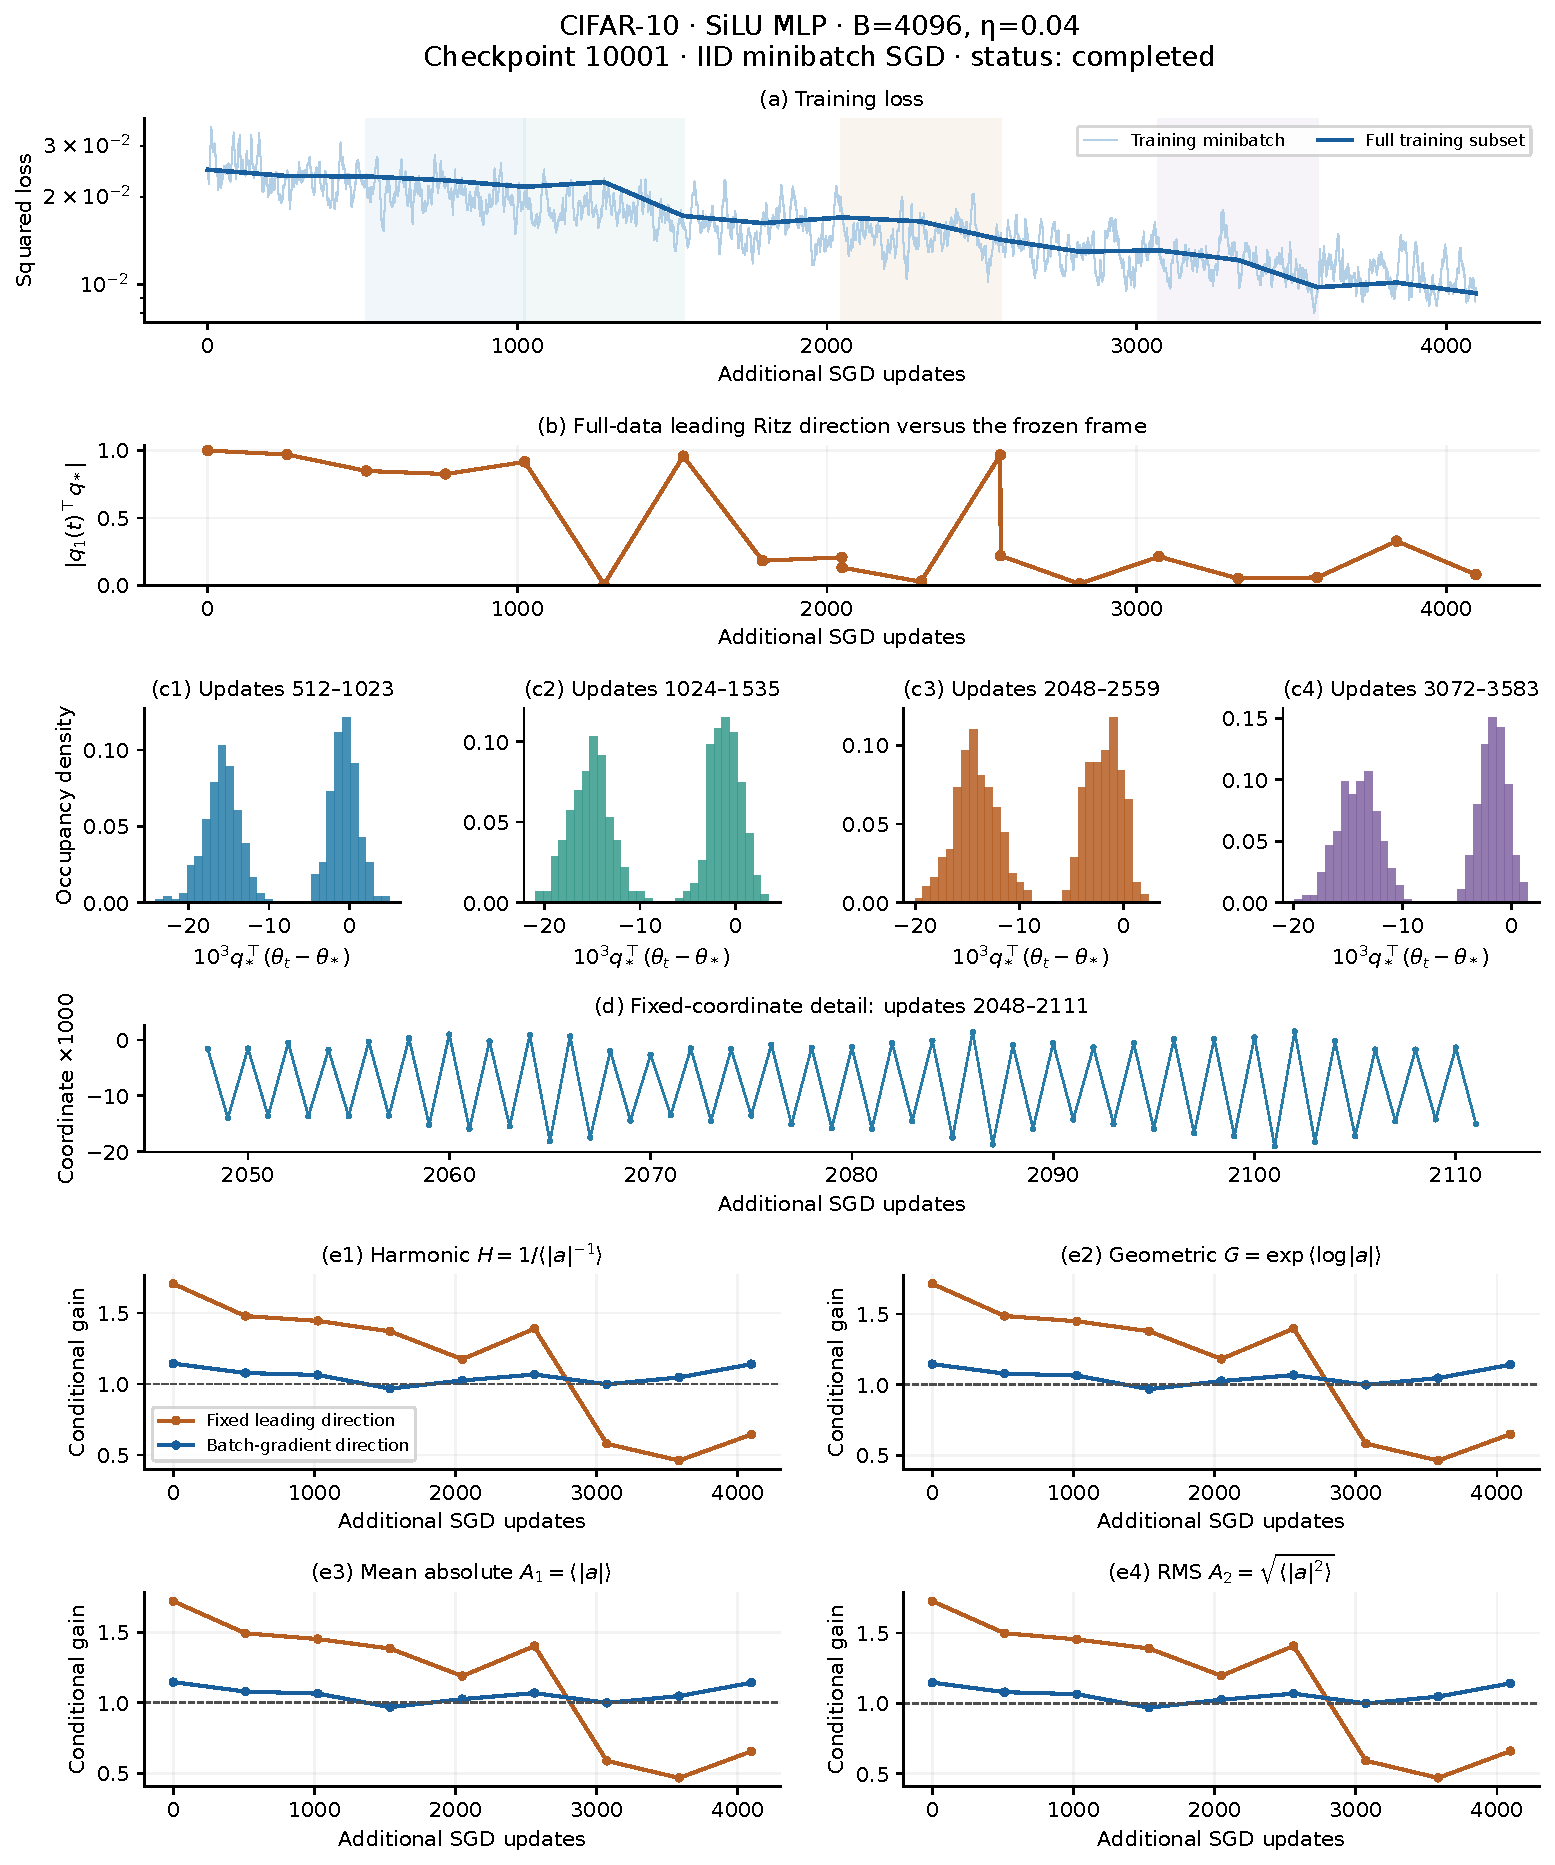
\includegraphics[width=\linewidth,height=0.77\textheight,keepaspectratio]{img/appendix_directional_ladders/mlp_silu_B4096_anchor_revised.pdf}
\caption{\textbf{SiLU MLP, batch 4096, learning rate 0.04, parent checkpoint 10001.} Loss is shown for both training minibatches and the full 8192-example training subset. The plotting direction $q_*$ and center $\theta_*$ stay fixed at the parent checkpoint; $\theta_*$ is not a verified minimizer. Alignment with separately recomputed leading Hessian Ritz vectors is measured on the full subset, not assumed. Four declared 512-update windows and one 64-update detail are displayed without selection by modality. The lower four panels show fresh conditional scalar gains, comparing $a_{*,B}=1-\eta q_*^\top H_Bq_*$ and $a_{g,B}=1-\eta g_B^\top H_Bg_B/(g_B^\top g_B)$. Their summaries are $H=1/\langle|a|^{-1}\rangle$, $G=\exp\langle\log|a|\rangle$, $A_1=\langle|a|\rangle$, and $A_2=\sqrt{\langle|a|^2\rangle}$, all with reference one. Except for the original anchor, each state has 64 fresh probes every256 updates; the anchor uses 128 probes initially and24 every512 updates. Only even-update states appear here; no phase-averaged or stationary claim follows. No inverse-gain floor is applied.}
\end{figure}\clearpage
\begin{figure}[p]\centering
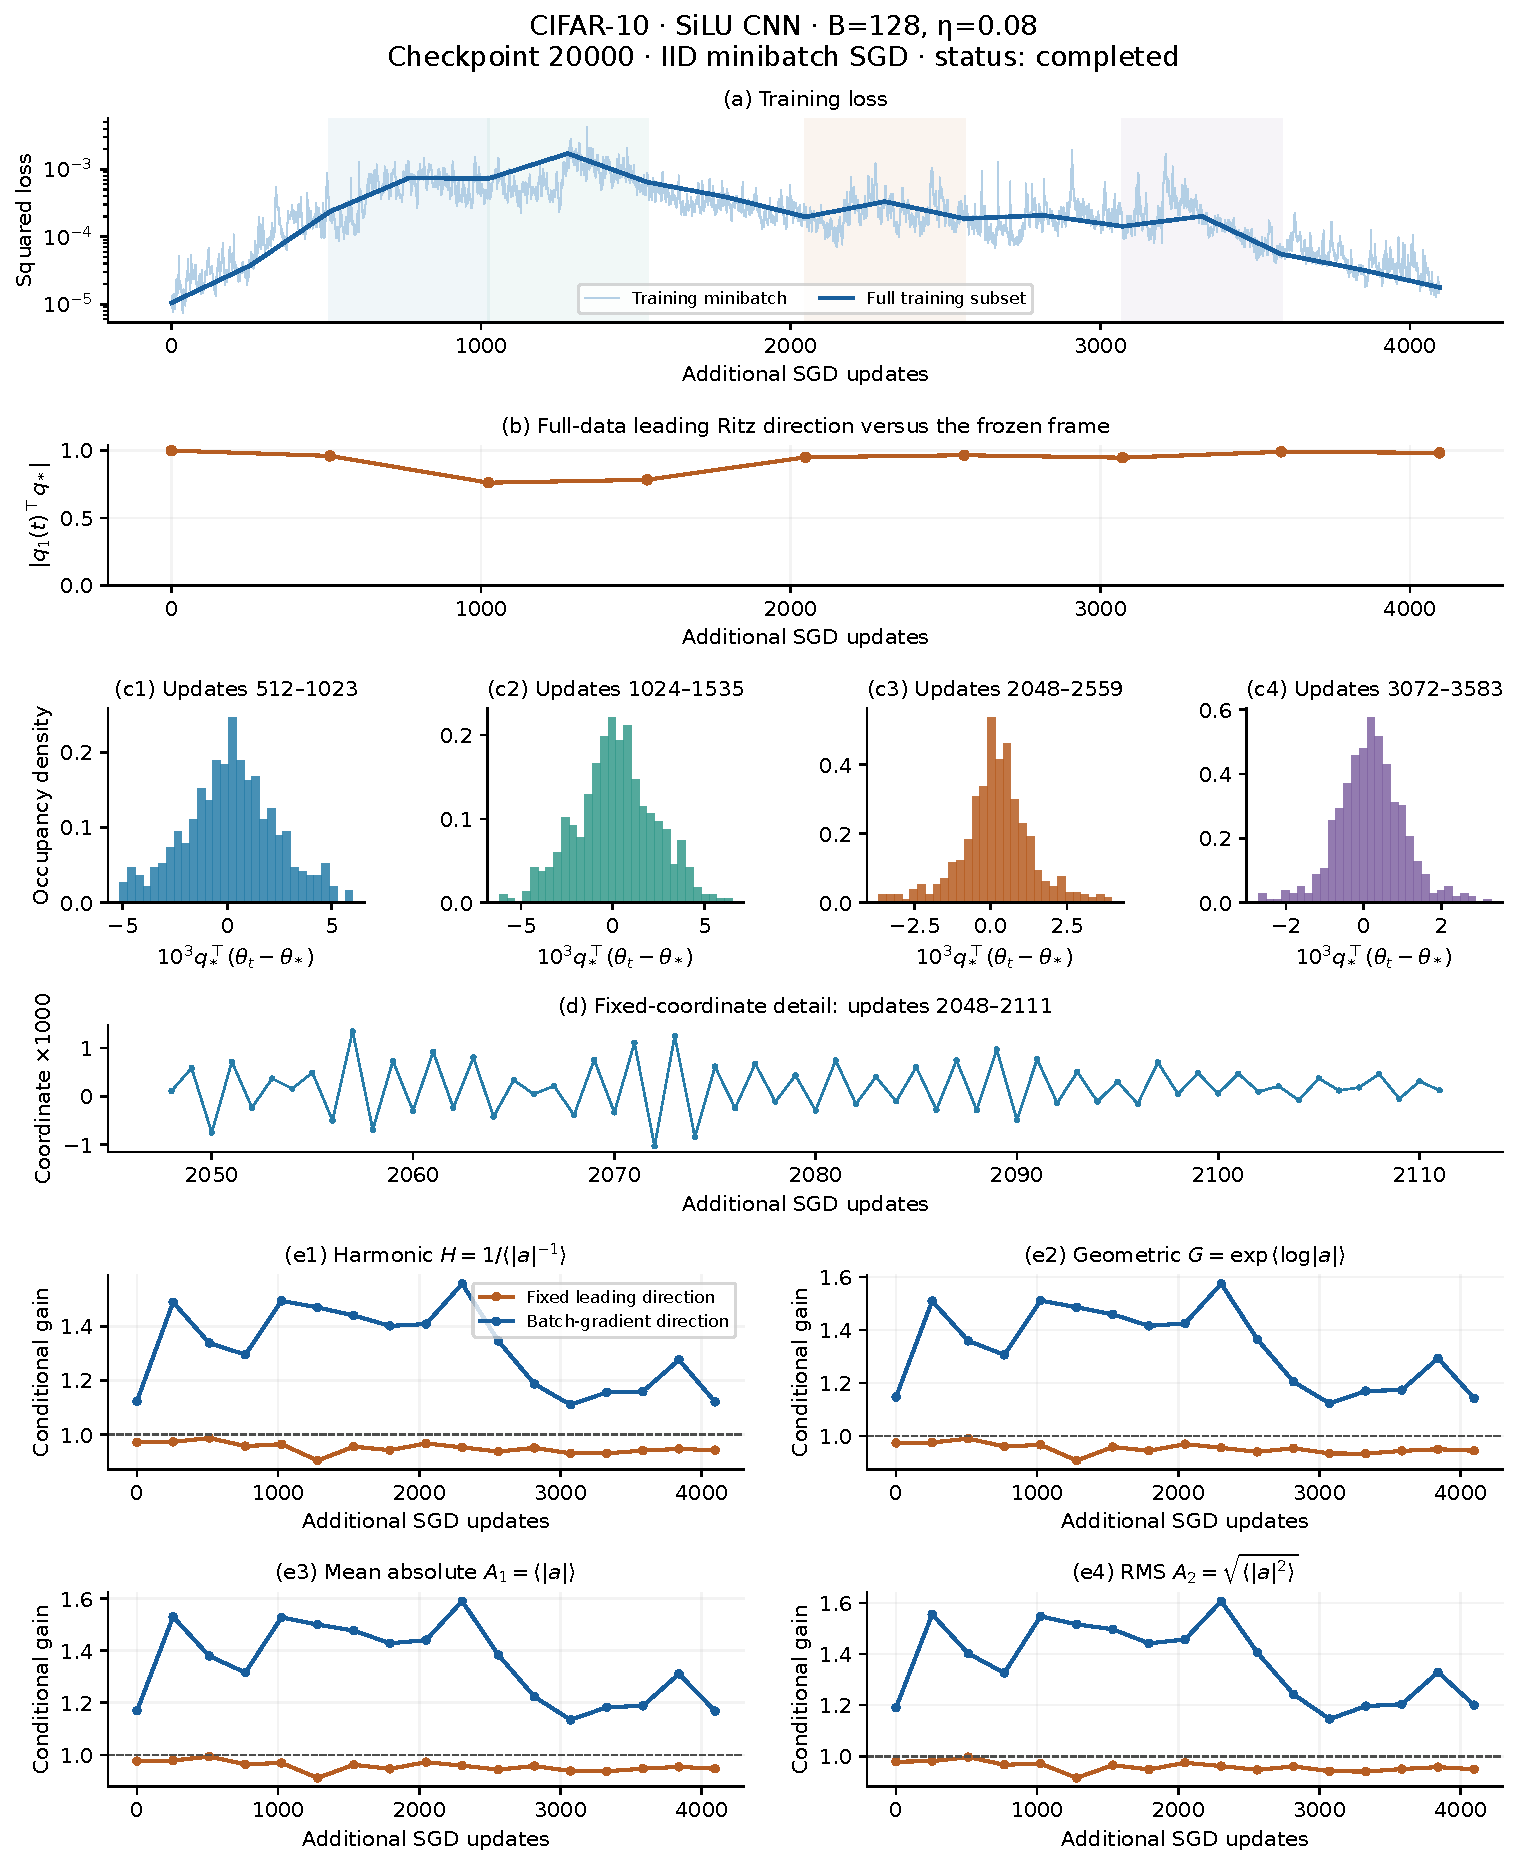
\includegraphics[width=\linewidth,height=0.77\textheight,keepaspectratio]{img/appendix_directional_ladders/cnn_silu_B128.pdf}
\caption{\textbf{SiLU CNN, batch 128, learning rate 0.08, parent checkpoint 20000.} Loss is shown for both training minibatches and the full 8192-example training subset. The plotting direction $q_*$ and center $\theta_*$ stay fixed at the parent checkpoint; $\theta_*$ is not a verified minimizer. Alignment with separately recomputed leading Hessian Ritz vectors is measured on the full subset, not assumed. Four declared 512-update windows and one 64-update detail are displayed without selection by modality. The lower four panels show fresh conditional scalar gains, comparing $a_{*,B}=1-\eta q_*^\top H_Bq_*$ and $a_{g,B}=1-\eta g_B^\top H_Bg_B/(g_B^\top g_B)$. Their summaries are $H=1/\langle|a|^{-1}\rangle$, $G=\exp\langle\log|a|\rangle$, $A_1=\langle|a|\rangle$, and $A_2=\sqrt{\langle|a|^2\rangle}$, all with reference one. Except for the original anchor, each state has 64 fresh probes every256 updates; the anchor uses 128 probes initially and24 every512 updates. Only even-update states appear here; no phase-averaged or stationary claim follows. No inverse-gain floor is applied.}
\end{figure}\clearpage
\begin{figure}[p]\centering
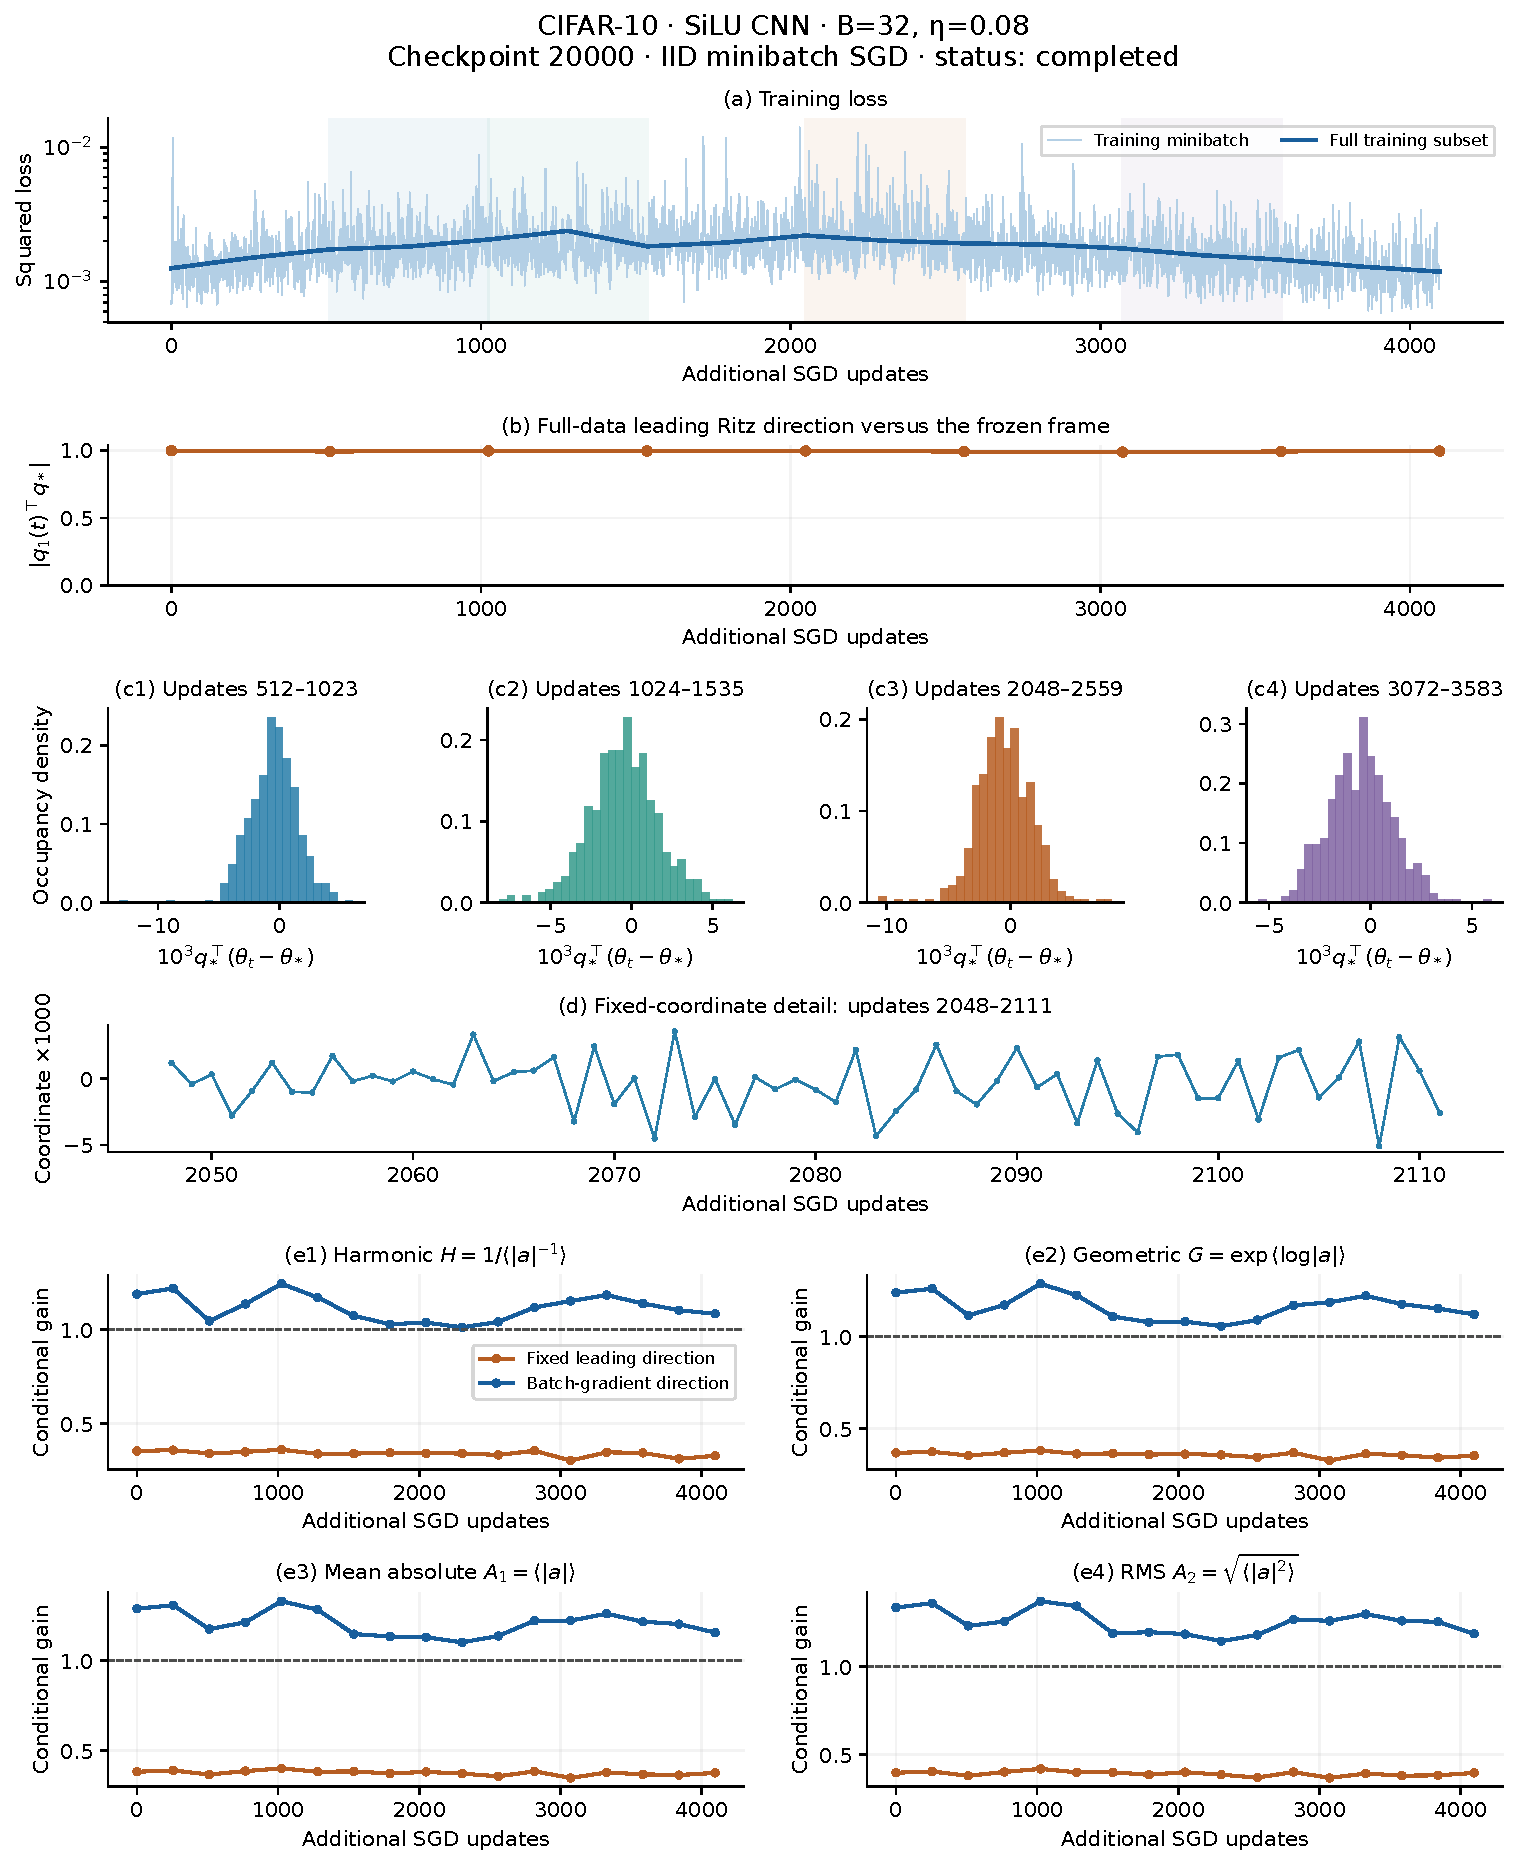
\includegraphics[width=\linewidth,height=0.77\textheight,keepaspectratio]{img/appendix_directional_ladders/cnn_silu_B32.pdf}
\caption{\textbf{SiLU CNN, batch 32, learning rate 0.08, parent checkpoint 20000.} Loss is shown for both training minibatches and the full 8192-example training subset. The plotting direction $q_*$ and center $\theta_*$ stay fixed at the parent checkpoint; $\theta_*$ is not a verified minimizer. Alignment with separately recomputed leading Hessian Ritz vectors is measured on the full subset, not assumed. Four declared 512-update windows and one 64-update detail are displayed without selection by modality. The lower four panels show fresh conditional scalar gains, comparing $a_{*,B}=1-\eta q_*^\top H_Bq_*$ and $a_{g,B}=1-\eta g_B^\top H_Bg_B/(g_B^\top g_B)$. Their summaries are $H=1/\langle|a|^{-1}\rangle$, $G=\exp\langle\log|a|\rangle$, $A_1=\langle|a|\rangle$, and $A_2=\sqrt{\langle|a|^2\rangle}$, all with reference one. Except for the original anchor, each state has 64 fresh probes every256 updates; the anchor uses 128 probes initially and24 every512 updates. Only even-update states appear here; no phase-averaged or stationary claim follows. No inverse-gain floor is applied.}
\end{figure}\clearpage
\begin{figure}[p]\centering
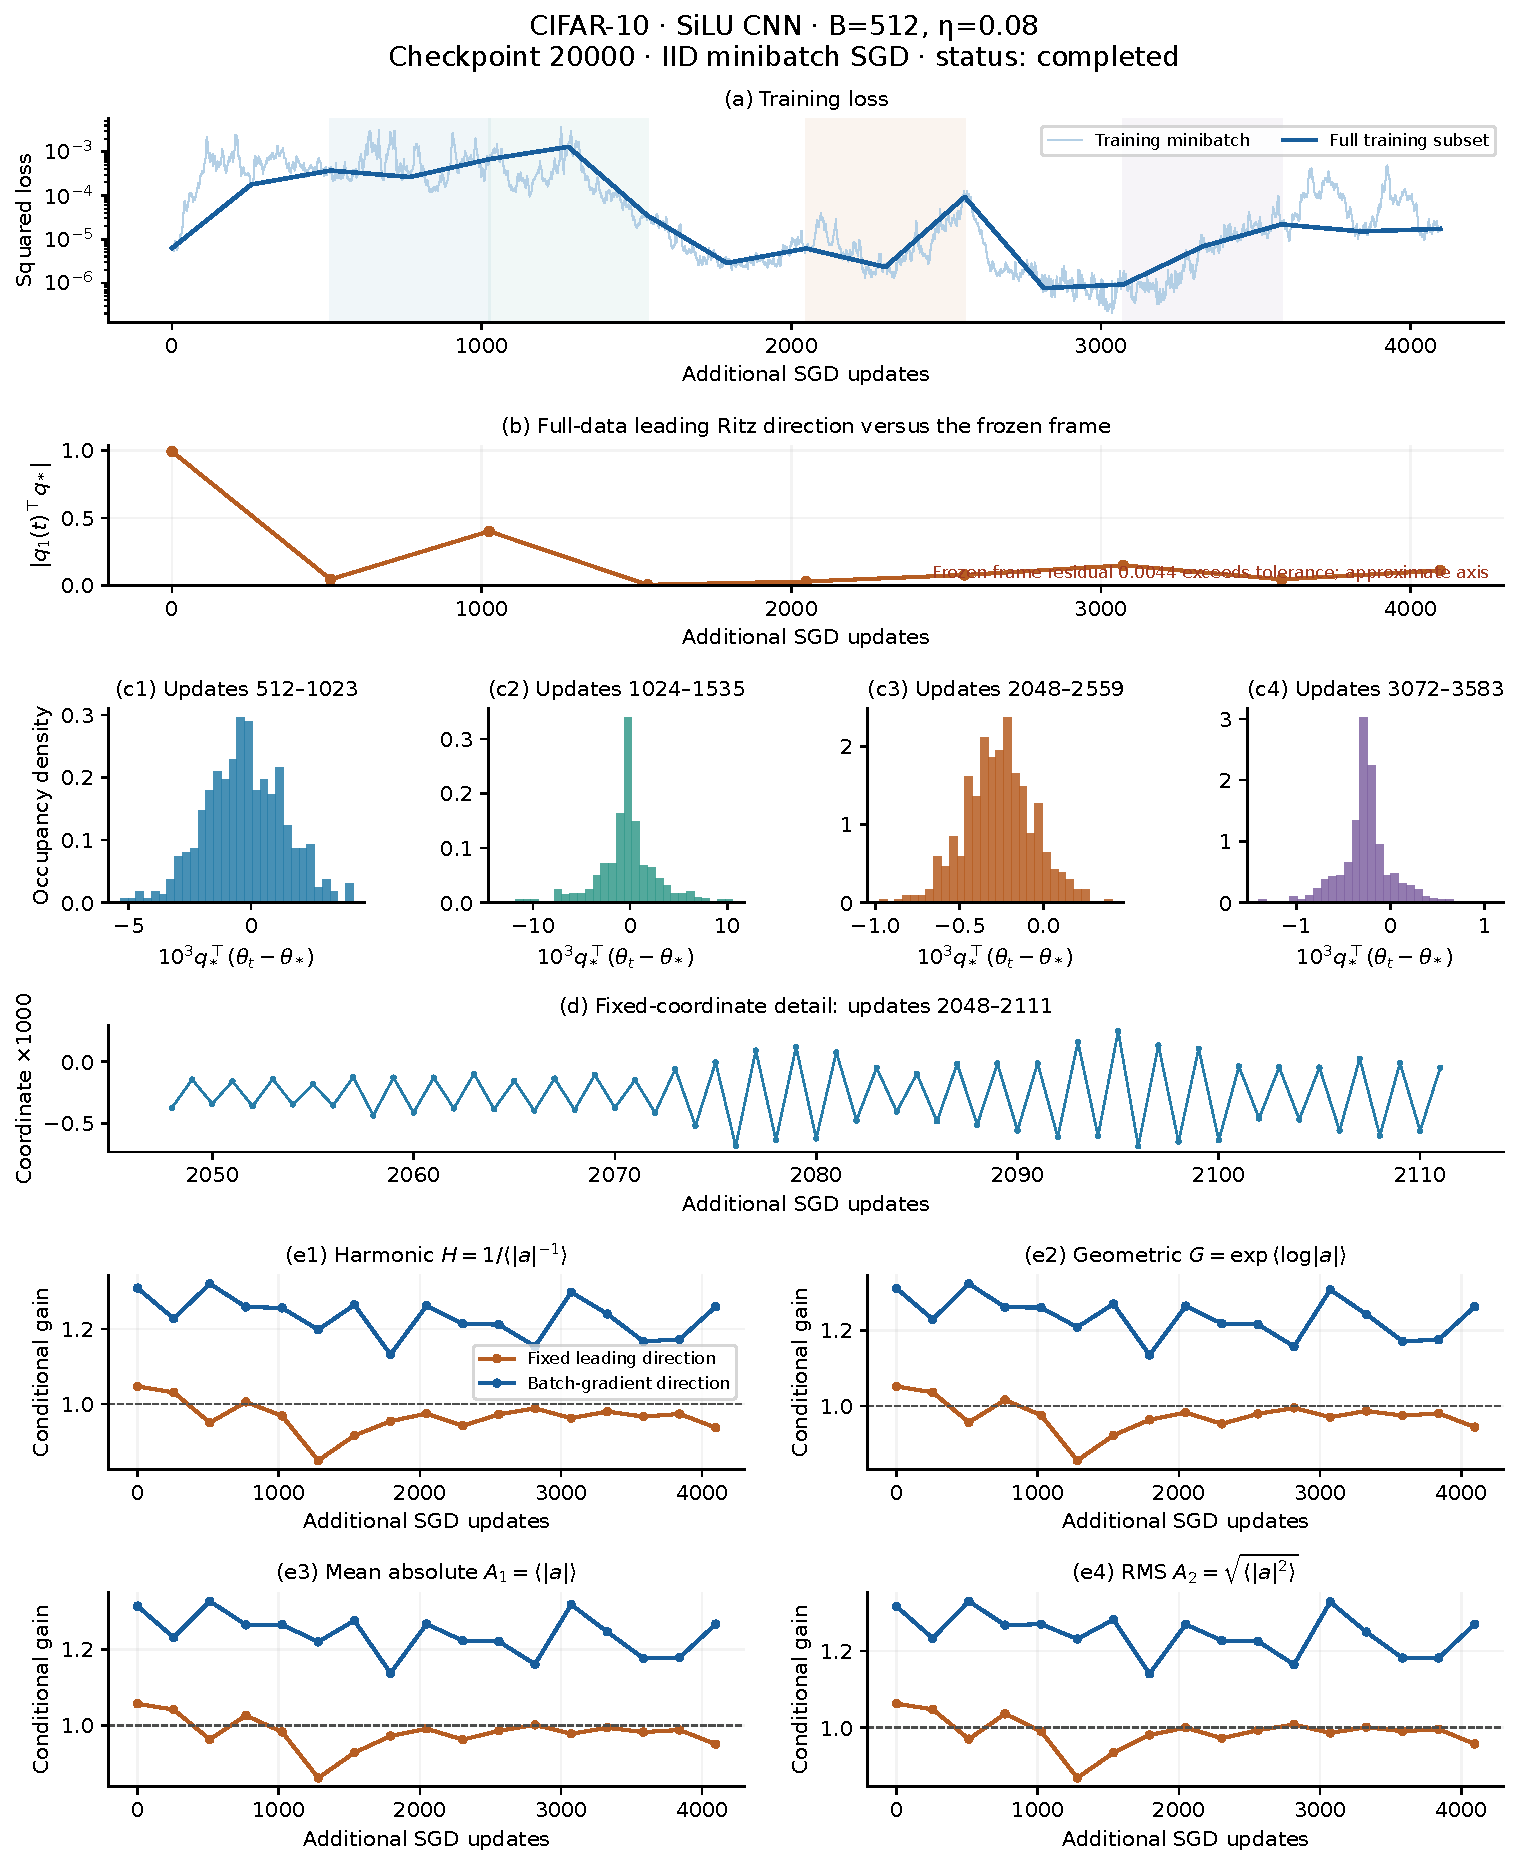
\includegraphics[width=\linewidth,height=0.77\textheight,keepaspectratio]{img/appendix_directional_ladders/cnn_silu_B512.pdf}
\caption{\textbf{SiLU CNN, batch 512, learning rate 0.08, parent checkpoint 20000.} Loss is shown for both training minibatches and the full 8192-example training subset. The plotting direction $q_*$ and center $\theta_*$ stay fixed at the parent checkpoint; $\theta_*$ is not a verified minimizer. Alignment with separately recomputed leading Hessian Ritz vectors is measured on the full subset, not assumed. Four declared 512-update windows and one 64-update detail are displayed without selection by modality. The lower four panels show fresh conditional scalar gains, comparing $a_{*,B}=1-\eta q_*^\top H_Bq_*$ and $a_{g,B}=1-\eta g_B^\top H_Bg_B/(g_B^\top g_B)$. Their summaries are $H=1/\langle|a|^{-1}\rangle$, $G=\exp\langle\log|a|\rangle$, $A_1=\langle|a|\rangle$, and $A_2=\sqrt{\langle|a|^2\rangle}$, all with reference one. Except for the original anchor, each state has 64 fresh probes every256 updates; the anchor uses 128 probes initially and24 every512 updates. Only even-update states appear here; no phase-averaged or stationary claim follows. No inverse-gain floor is applied.}
\end{figure}\clearpage
\begin{figure}[p]\centering
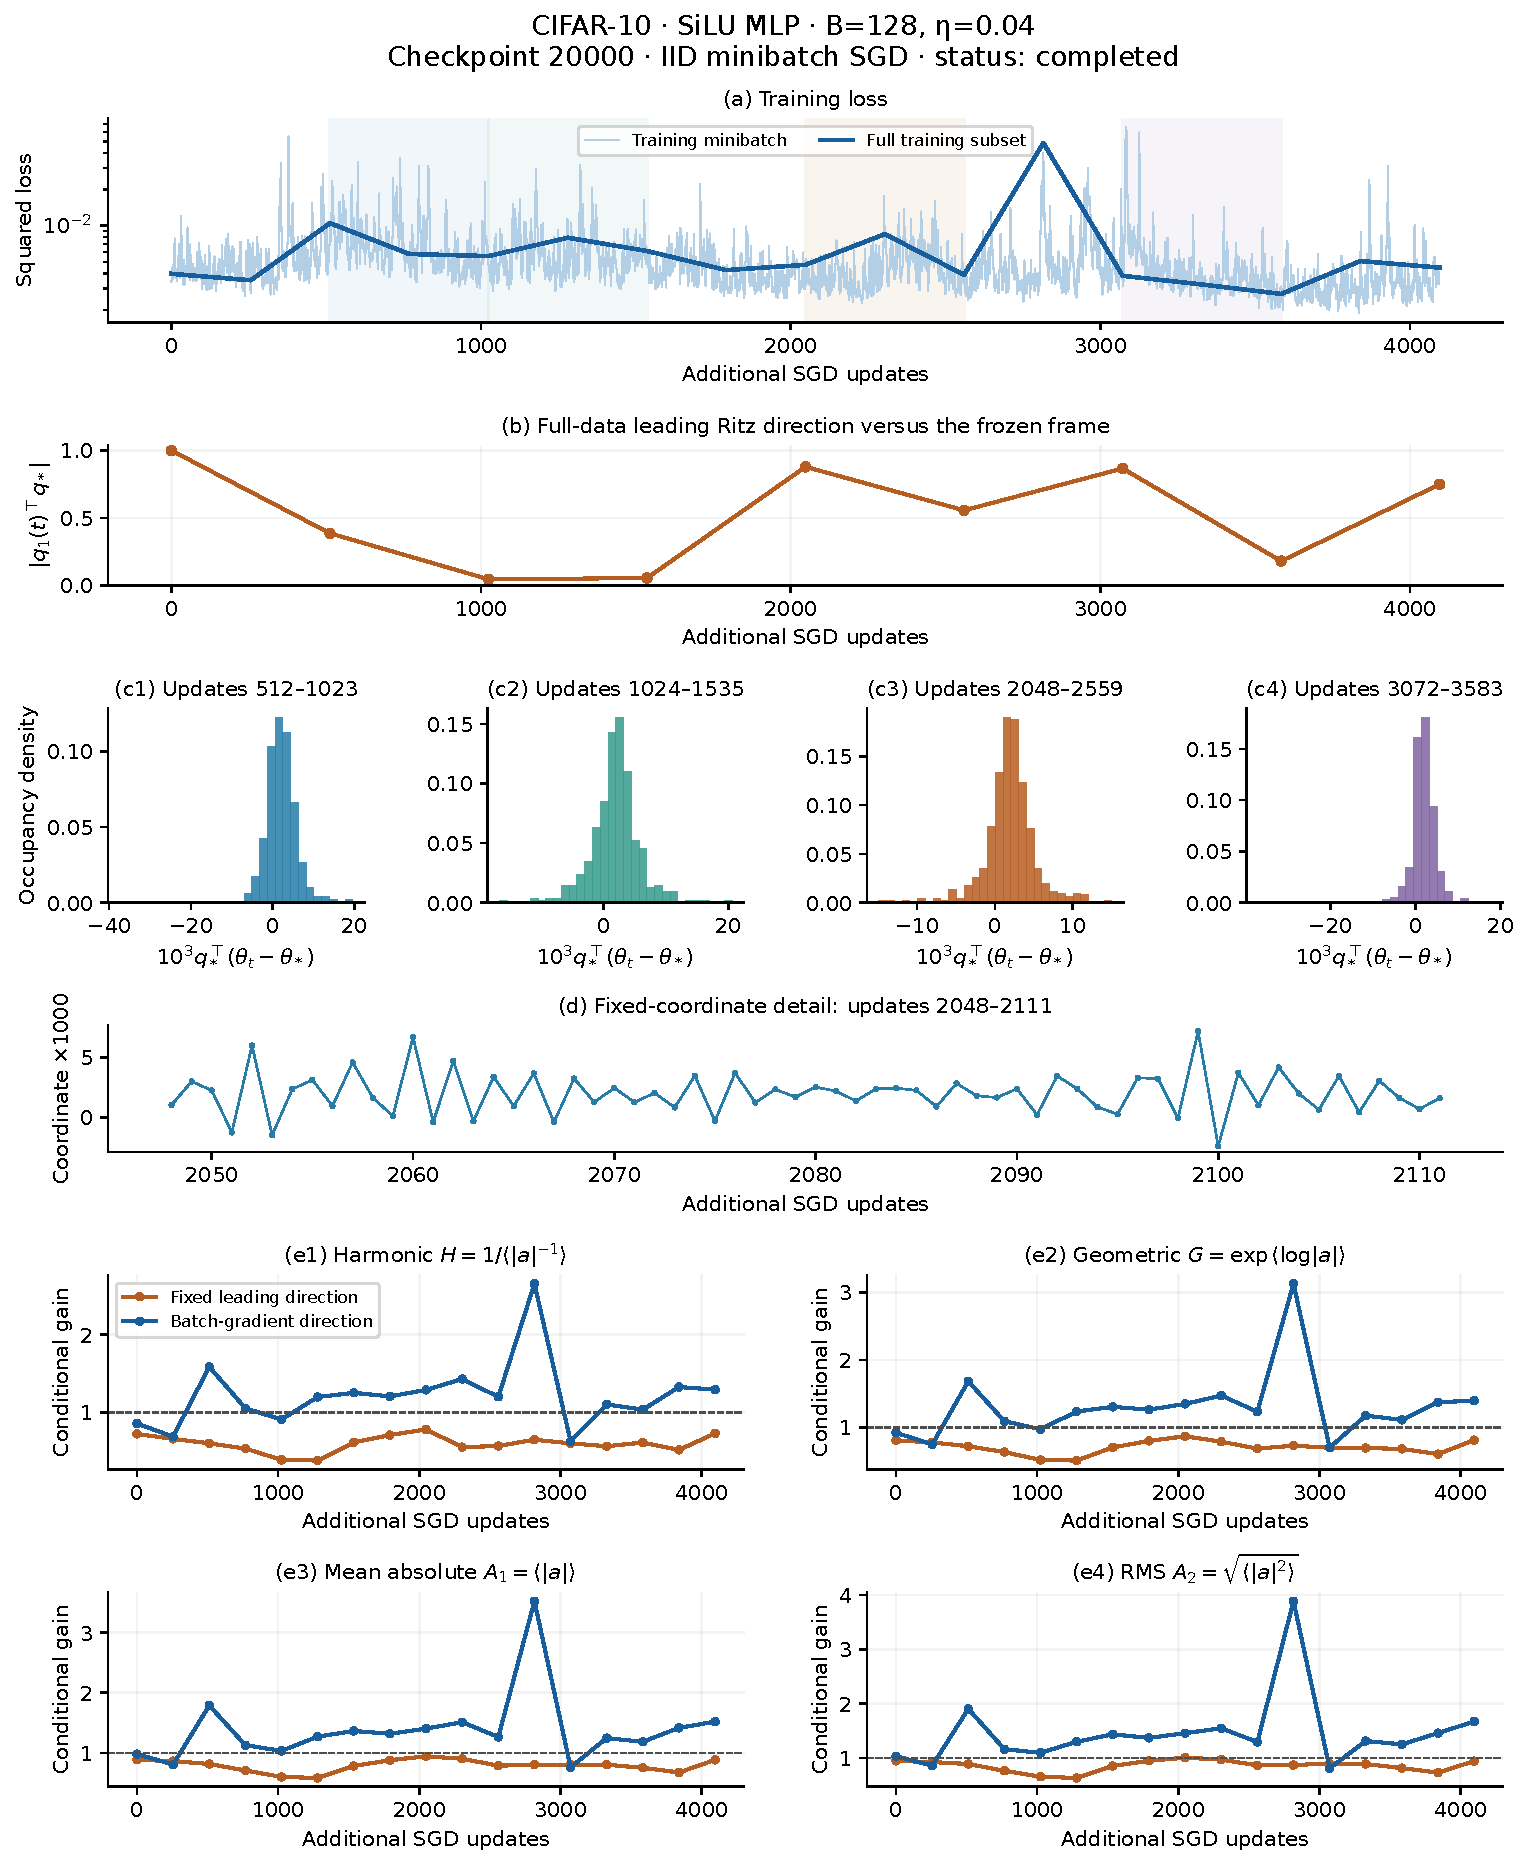
\includegraphics[width=\linewidth,height=0.77\textheight,keepaspectratio]{img/appendix_directional_ladders/mlp_silu_B128.pdf}
\caption{\textbf{SiLU MLP, batch 128, learning rate 0.04, parent checkpoint 20000.} Loss is shown for both training minibatches and the full 8192-example training subset. The plotting direction $q_*$ and center $\theta_*$ stay fixed at the parent checkpoint; $\theta_*$ is not a verified minimizer. Alignment with separately recomputed leading Hessian Ritz vectors is measured on the full subset, not assumed. Four declared 512-update windows and one 64-update detail are displayed without selection by modality. The lower four panels show fresh conditional scalar gains, comparing $a_{*,B}=1-\eta q_*^\top H_Bq_*$ and $a_{g,B}=1-\eta g_B^\top H_Bg_B/(g_B^\top g_B)$. Their summaries are $H=1/\langle|a|^{-1}\rangle$, $G=\exp\langle\log|a|\rangle$, $A_1=\langle|a|\rangle$, and $A_2=\sqrt{\langle|a|^2\rangle}$, all with reference one. Except for the original anchor, each state has 64 fresh probes every256 updates; the anchor uses 128 probes initially and24 every512 updates. Only even-update states appear here; no phase-averaged or stationary claim follows. No inverse-gain floor is applied.}
\end{figure}\clearpage
\begin{figure}[p]\centering
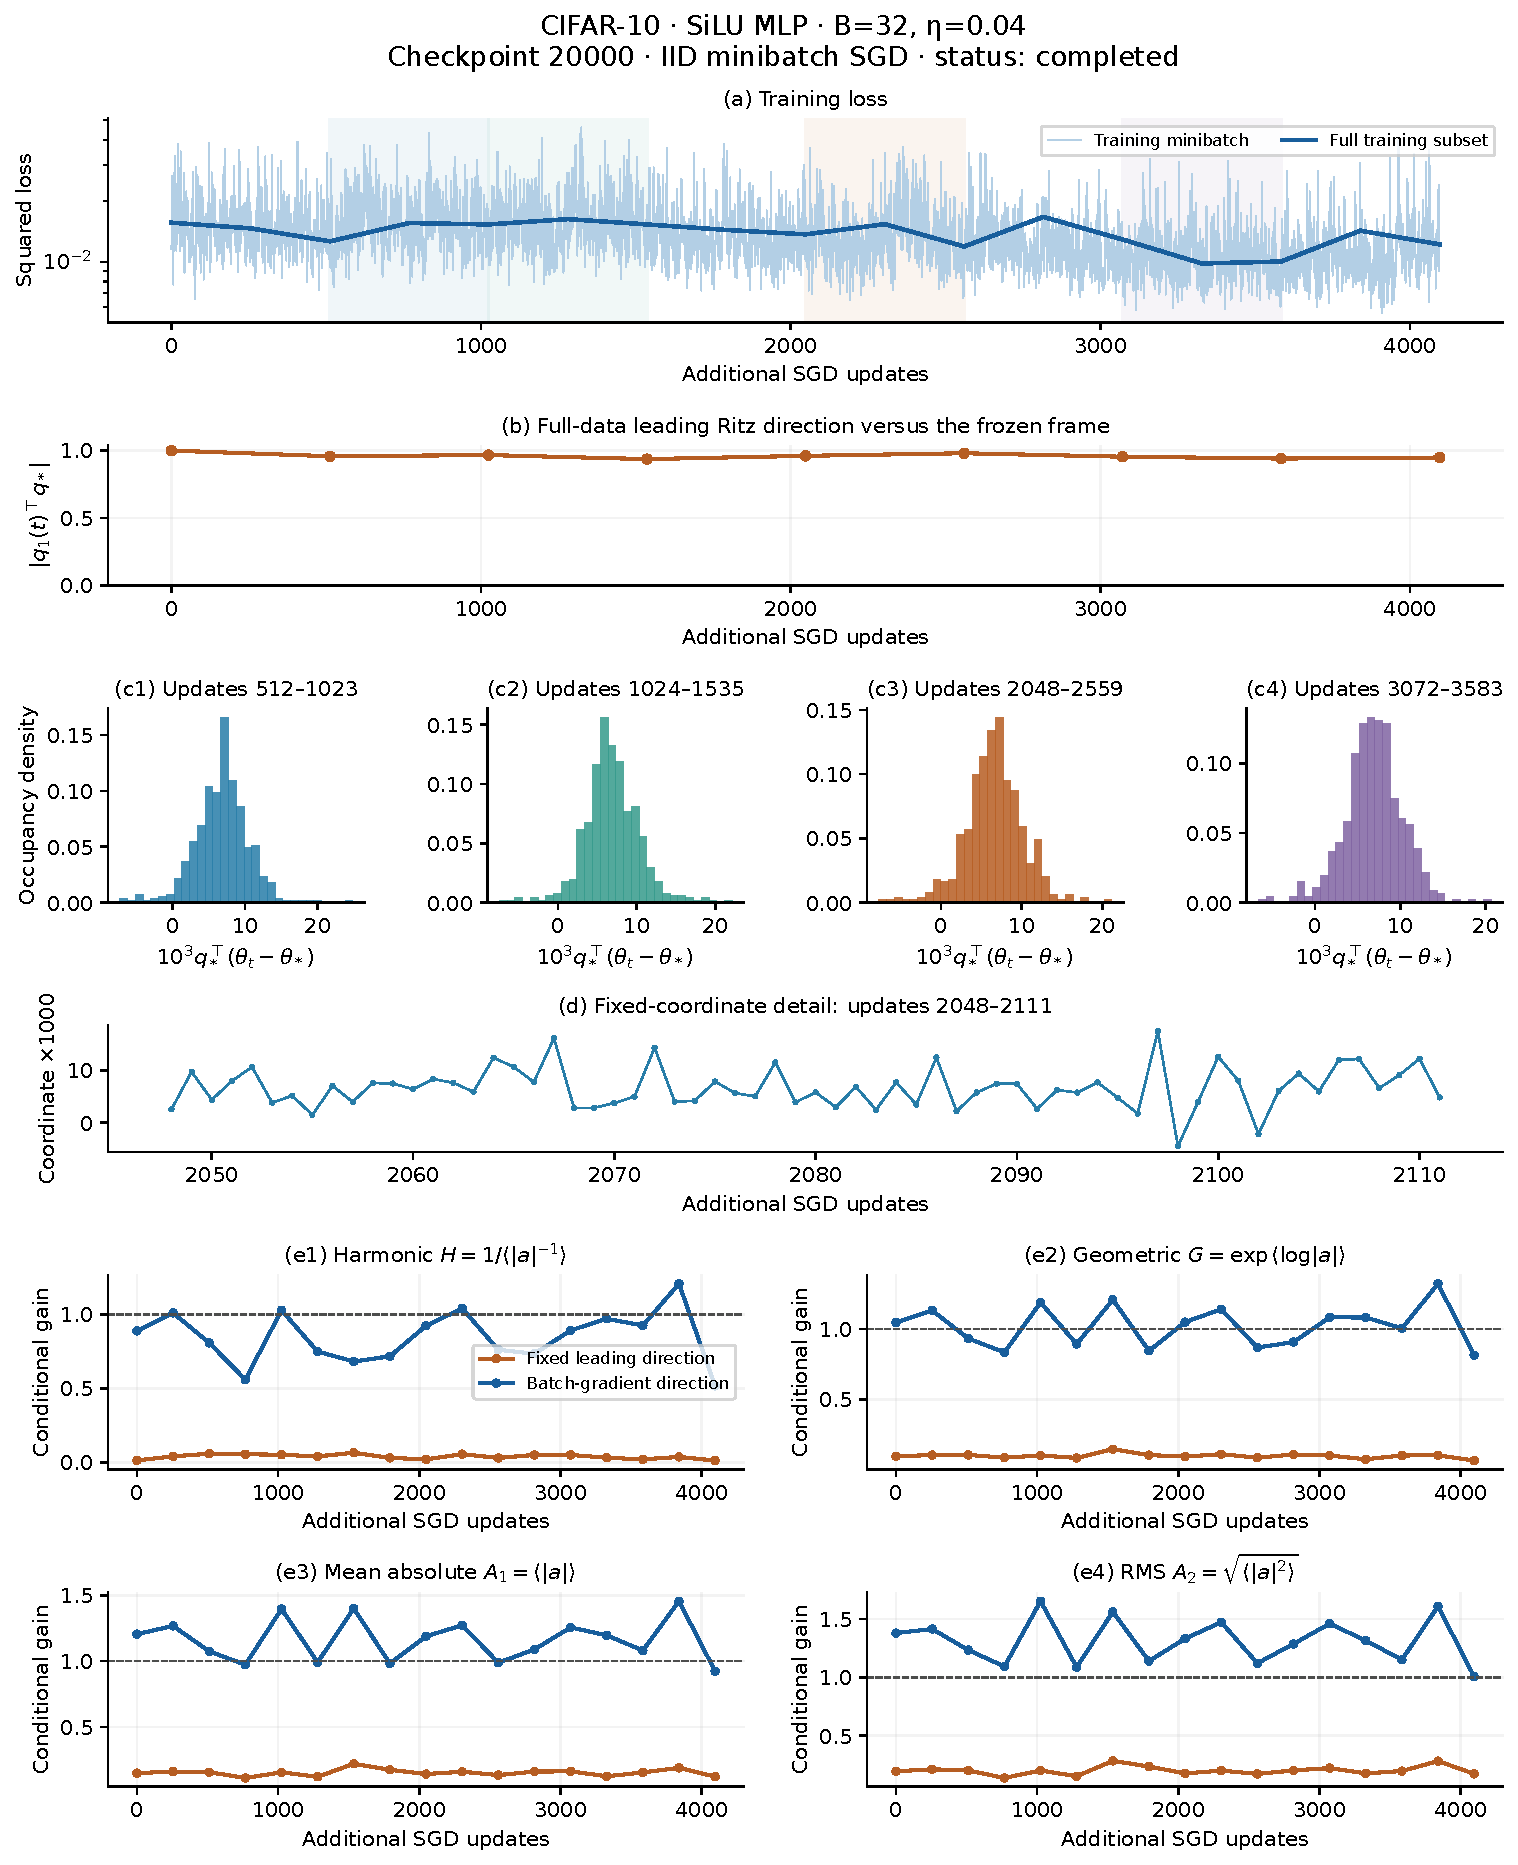
\includegraphics[width=\linewidth,height=0.77\textheight,keepaspectratio]{img/appendix_directional_ladders/mlp_silu_B32.pdf}
\caption{\textbf{SiLU MLP, batch 32, learning rate 0.04, parent checkpoint 20000.} Loss is shown for both training minibatches and the full 8192-example training subset. The plotting direction $q_*$ and center $\theta_*$ stay fixed at the parent checkpoint; $\theta_*$ is not a verified minimizer. Alignment with separately recomputed leading Hessian Ritz vectors is measured on the full subset, not assumed. Four declared 512-update windows and one 64-update detail are displayed without selection by modality. The lower four panels show fresh conditional scalar gains, comparing $a_{*,B}=1-\eta q_*^\top H_Bq_*$ and $a_{g,B}=1-\eta g_B^\top H_Bg_B/(g_B^\top g_B)$. Their summaries are $H=1/\langle|a|^{-1}\rangle$, $G=\exp\langle\log|a|\rangle$, $A_1=\langle|a|\rangle$, and $A_2=\sqrt{\langle|a|^2\rangle}$, all with reference one. Except for the original anchor, each state has 64 fresh probes every256 updates; the anchor uses 128 probes initially and24 every512 updates. Only even-update states appear here; no phase-averaged or stationary claim follows. No inverse-gain floor is applied.}
\end{figure}\clearpage
\begin{figure}[p]\centering
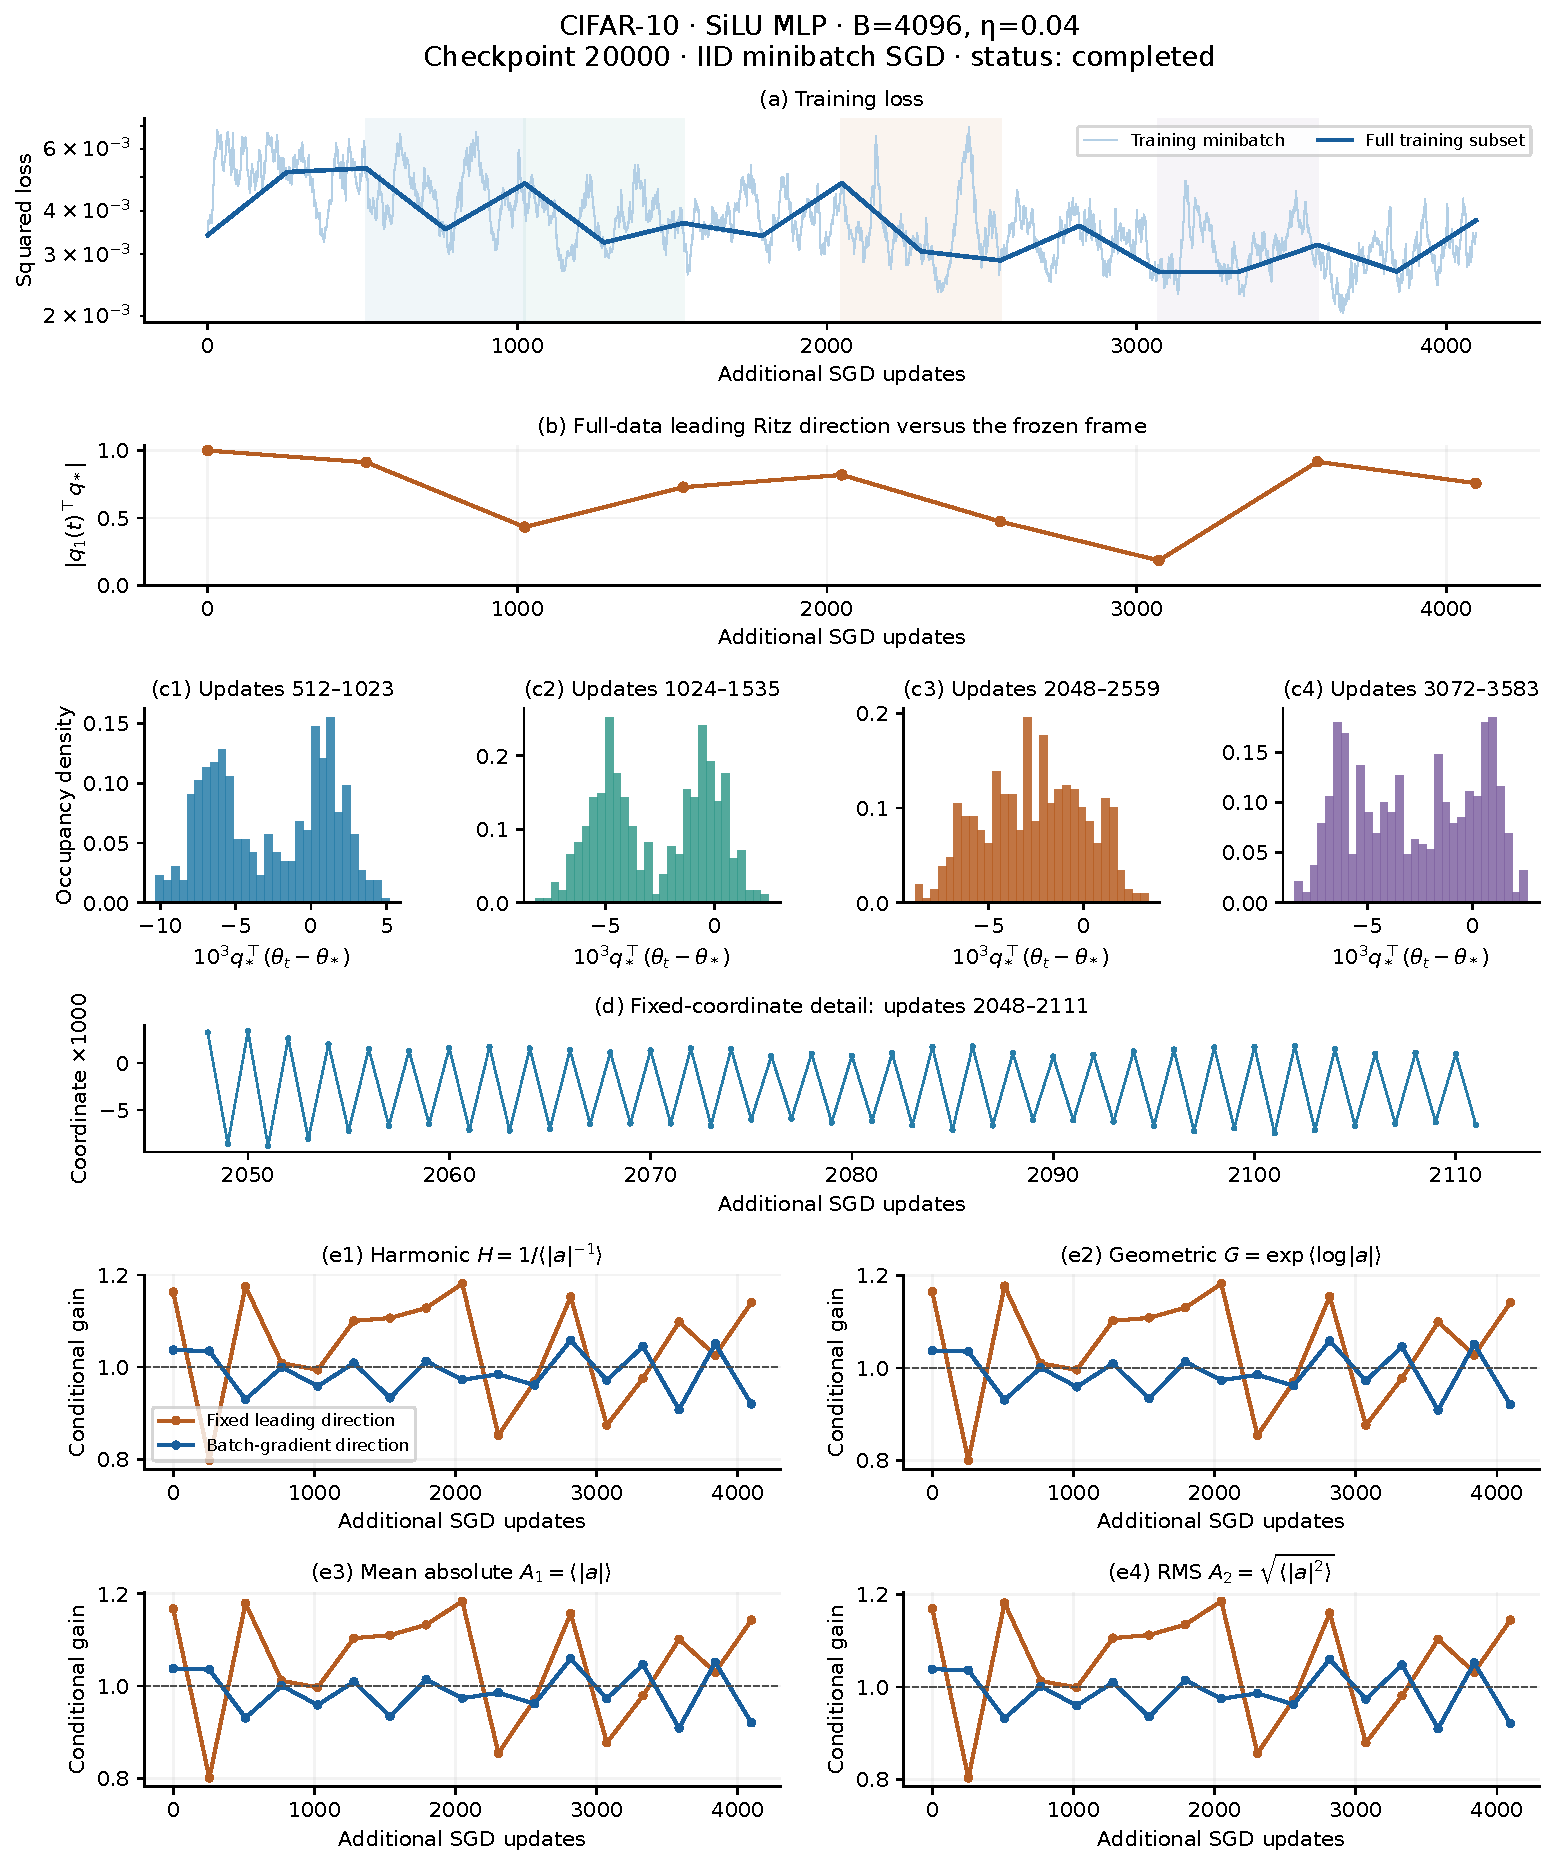
\includegraphics[width=\linewidth,height=0.77\textheight,keepaspectratio]{img/appendix_directional_ladders/mlp_silu_B4096.pdf}
\caption{\textbf{SiLU MLP, batch 4096, learning rate 0.04, parent checkpoint 20000.} Loss is shown for both training minibatches and the full 8192-example training subset. The plotting direction $q_*$ and center $\theta_*$ stay fixed at the parent checkpoint; $\theta_*$ is not a verified minimizer. Alignment with separately recomputed leading Hessian Ritz vectors is measured on the full subset, not assumed. Four declared 512-update windows and one 64-update detail are displayed without selection by modality. The lower four panels show fresh conditional scalar gains, comparing $a_{*,B}=1-\eta q_*^\top H_Bq_*$ and $a_{g,B}=1-\eta g_B^\top H_Bg_B/(g_B^\top g_B)$. Their summaries are $H=1/\langle|a|^{-1}\rangle$, $G=\exp\langle\log|a|\rangle$, $A_1=\langle|a|\rangle$, and $A_2=\sqrt{\langle|a|^2\rangle}$, all with reference one. Except for the original anchor, each state has 64 fresh probes every256 updates; the anchor uses 128 probes initially and24 every512 updates. Only even-update states appear here; no phase-averaged or stationary claim follows. No inverse-gain floor is applied.}
\end{figure}\clearpage
\begin{figure}[p]\centering
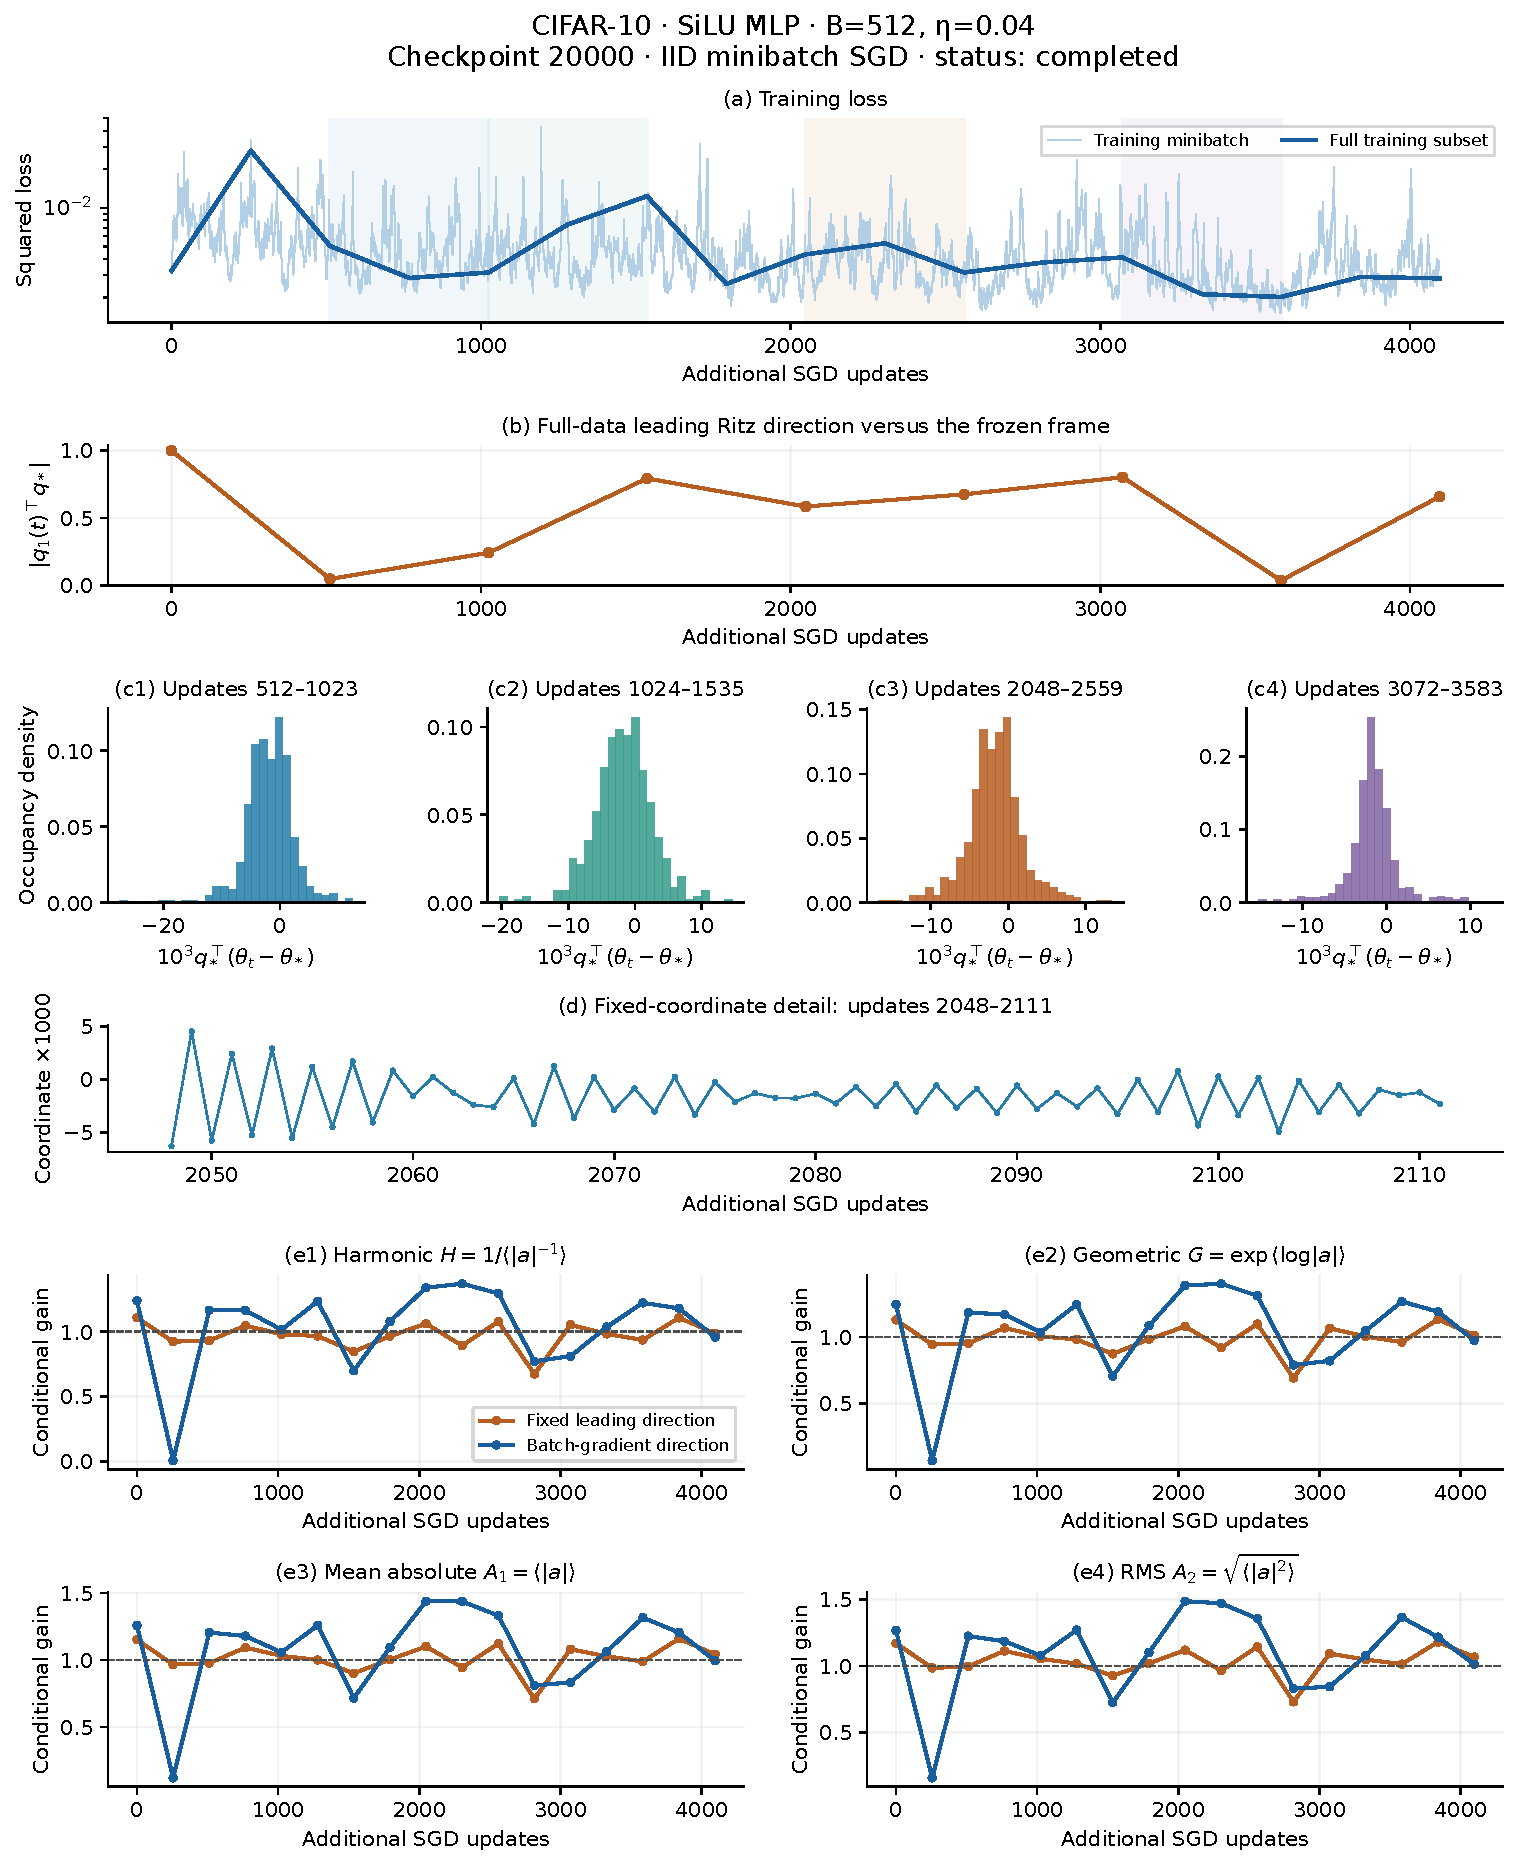
\includegraphics[width=\linewidth,height=0.77\textheight,keepaspectratio]{img/appendix_directional_ladders/mlp_silu_B512.pdf}
\caption{\textbf{SiLU MLP, batch 512, learning rate 0.04, parent checkpoint 20000.} Loss is shown for both training minibatches and the full 8192-example training subset. The plotting direction $q_*$ and center $\theta_*$ stay fixed at the parent checkpoint; $\theta_*$ is not a verified minimizer. Alignment with separately recomputed leading Hessian Ritz vectors is measured on the full subset, not assumed. Four declared 512-update windows and one 64-update detail are displayed without selection by modality. The lower four panels show fresh conditional scalar gains, comparing $a_{*,B}=1-\eta q_*^\top H_Bq_*$ and $a_{g,B}=1-\eta g_B^\top H_Bg_B/(g_B^\top g_B)$. Their summaries are $H=1/\langle|a|^{-1}\rangle$, $G=\exp\langle\log|a|\rangle$, $A_1=\langle|a|\rangle$, and $A_2=\sqrt{\langle|a|^2\rangle}$, all with reference one. Except for the original anchor, each state has 64 fresh probes every256 updates; the anchor uses 128 probes initially and24 every512 updates. Only even-update states appear here; no phase-averaged or stationary claim follows. No inverse-gain floor is applied.}
\end{figure}\clearpage
\begin{figure}[p]\centering
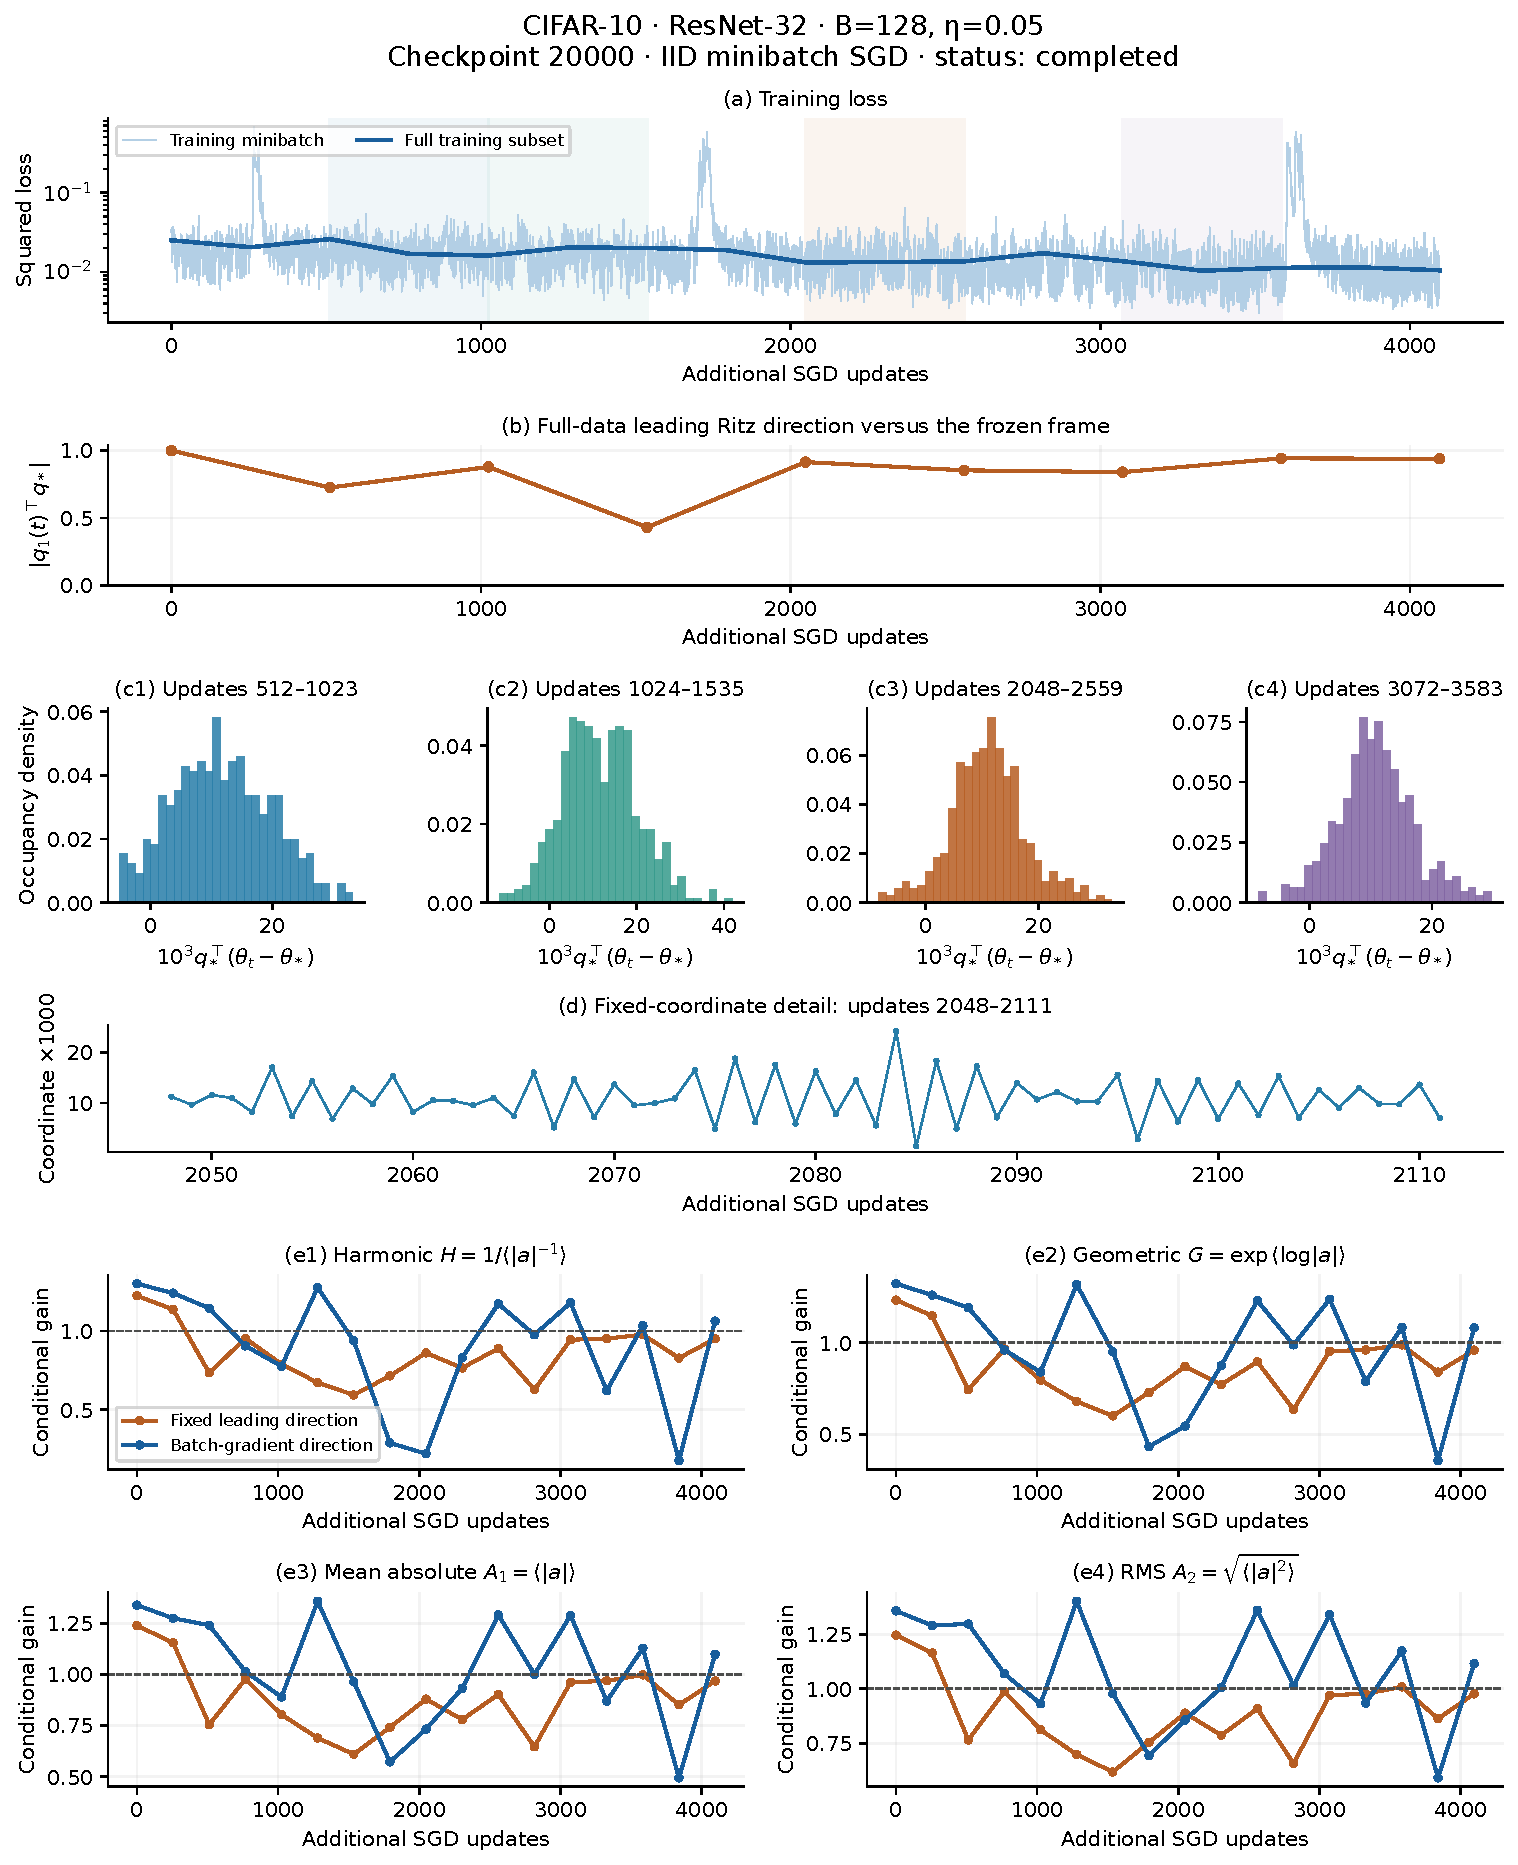
\includegraphics[width=\linewidth,height=0.77\textheight,keepaspectratio]{img/appendix_directional_ladders/resnet32_B128.pdf}
\caption{\textbf{ResNet-32, batch 128, learning rate 0.05, parent checkpoint 20000.} Loss is shown for both training minibatches and the full 8192-example training subset. The plotting direction $q_*$ and center $\theta_*$ stay fixed at the parent checkpoint; $\theta_*$ is not a verified minimizer. Alignment with separately recomputed leading Hessian Ritz vectors is measured on the full subset, not assumed. Four declared 512-update windows and one 64-update detail are displayed without selection by modality. The lower four panels show fresh conditional scalar gains, comparing $a_{*,B}=1-\eta q_*^\top H_Bq_*$ and $a_{g,B}=1-\eta g_B^\top H_Bg_B/(g_B^\top g_B)$. Their summaries are $H=1/\langle|a|^{-1}\rangle$, $G=\exp\langle\log|a|\rangle$, $A_1=\langle|a|\rangle$, and $A_2=\sqrt{\langle|a|^2\rangle}$, all with reference one. Except for the original anchor, each state has 64 fresh probes every256 updates; the anchor uses 128 probes initially and24 every512 updates. Only even-update states appear here; no phase-averaged or stationary claim follows. No inverse-gain floor is applied.}
\end{figure}\clearpage
\begin{figure}[p]\centering
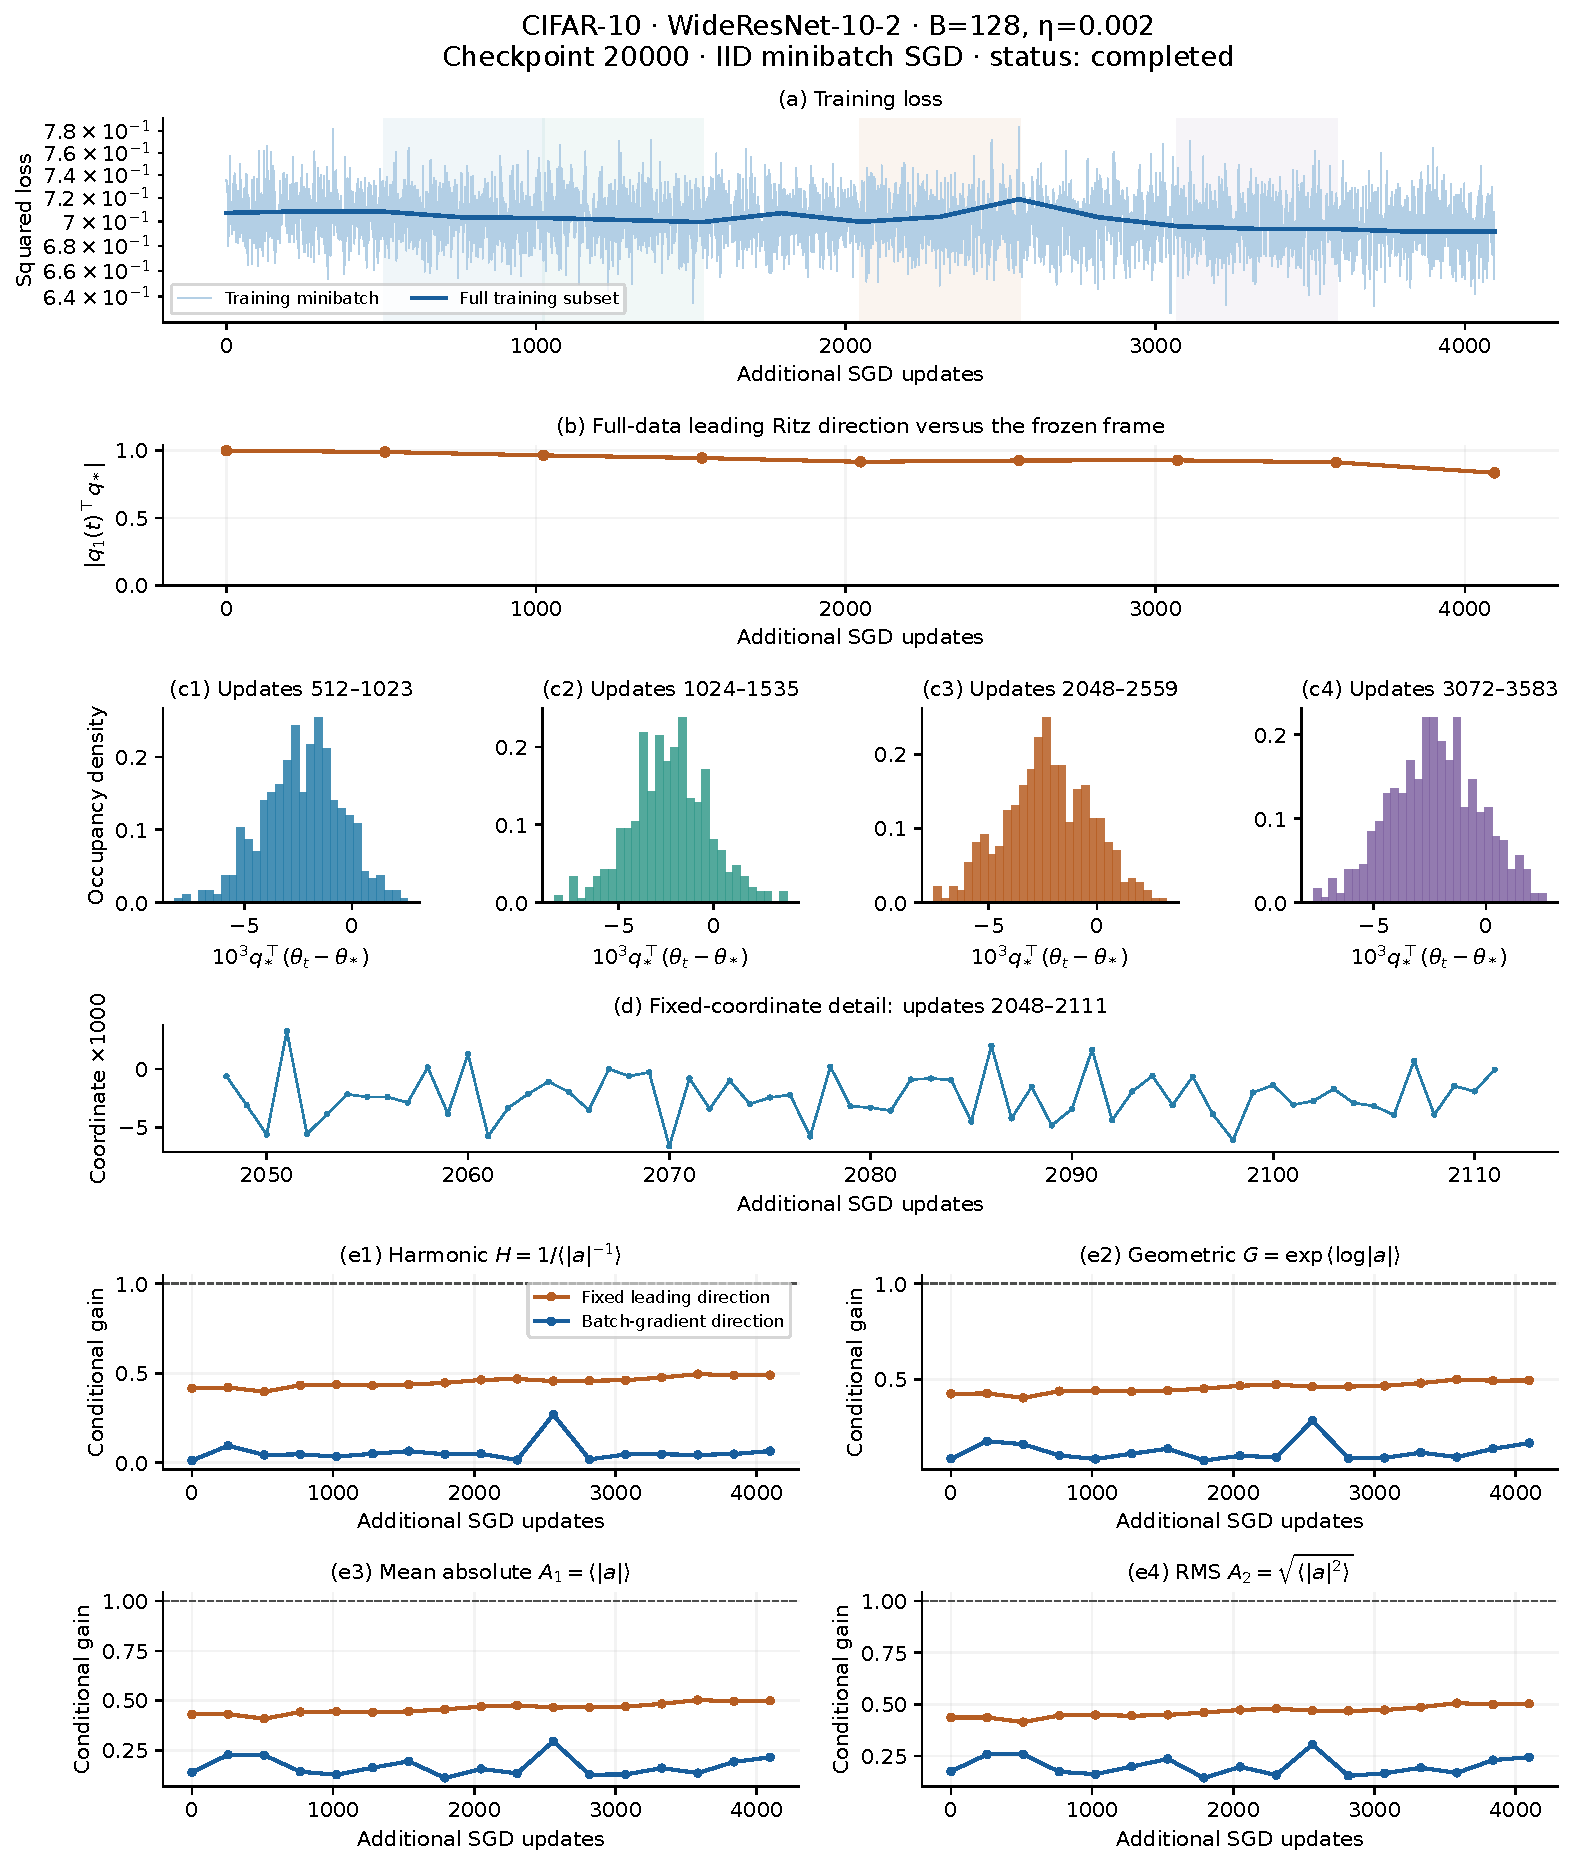
\includegraphics[width=\linewidth,height=0.77\textheight,keepaspectratio]{img/appendix_directional_ladders/wrn_no_bn_B128.pdf}
\caption{\textbf{WideResNet-10-2, batch 128, learning rate 0.002, parent checkpoint 20000.} Loss is shown for both training minibatches and the full 8192-example training subset. The plotting direction $q_*$ and center $\theta_*$ stay fixed at the parent checkpoint; $\theta_*$ is not a verified minimizer. Alignment with separately recomputed leading Hessian Ritz vectors is measured on the full subset, not assumed. Four declared 512-update windows and one 64-update detail are displayed without selection by modality. The lower four panels show fresh conditional scalar gains, comparing $a_{*,B}=1-\eta q_*^\top H_Bq_*$ and $a_{g,B}=1-\eta g_B^\top H_Bg_B/(g_B^\top g_B)$. Their summaries are $H=1/\langle|a|^{-1}\rangle$, $G=\exp\langle\log|a|\rangle$, $A_1=\langle|a|\rangle$, and $A_2=\sqrt{\langle|a|^2\rangle}$, all with reference one. Except for the original anchor, each state has 64 fresh probes every256 updates; the anchor uses 128 probes initially and24 every512 updates. Only even-update states appear here; no phase-averaged or stationary claim follows. No inverse-gain floor is applied.}
\end{figure}\clearpage
\begin{figure}[p]\centering
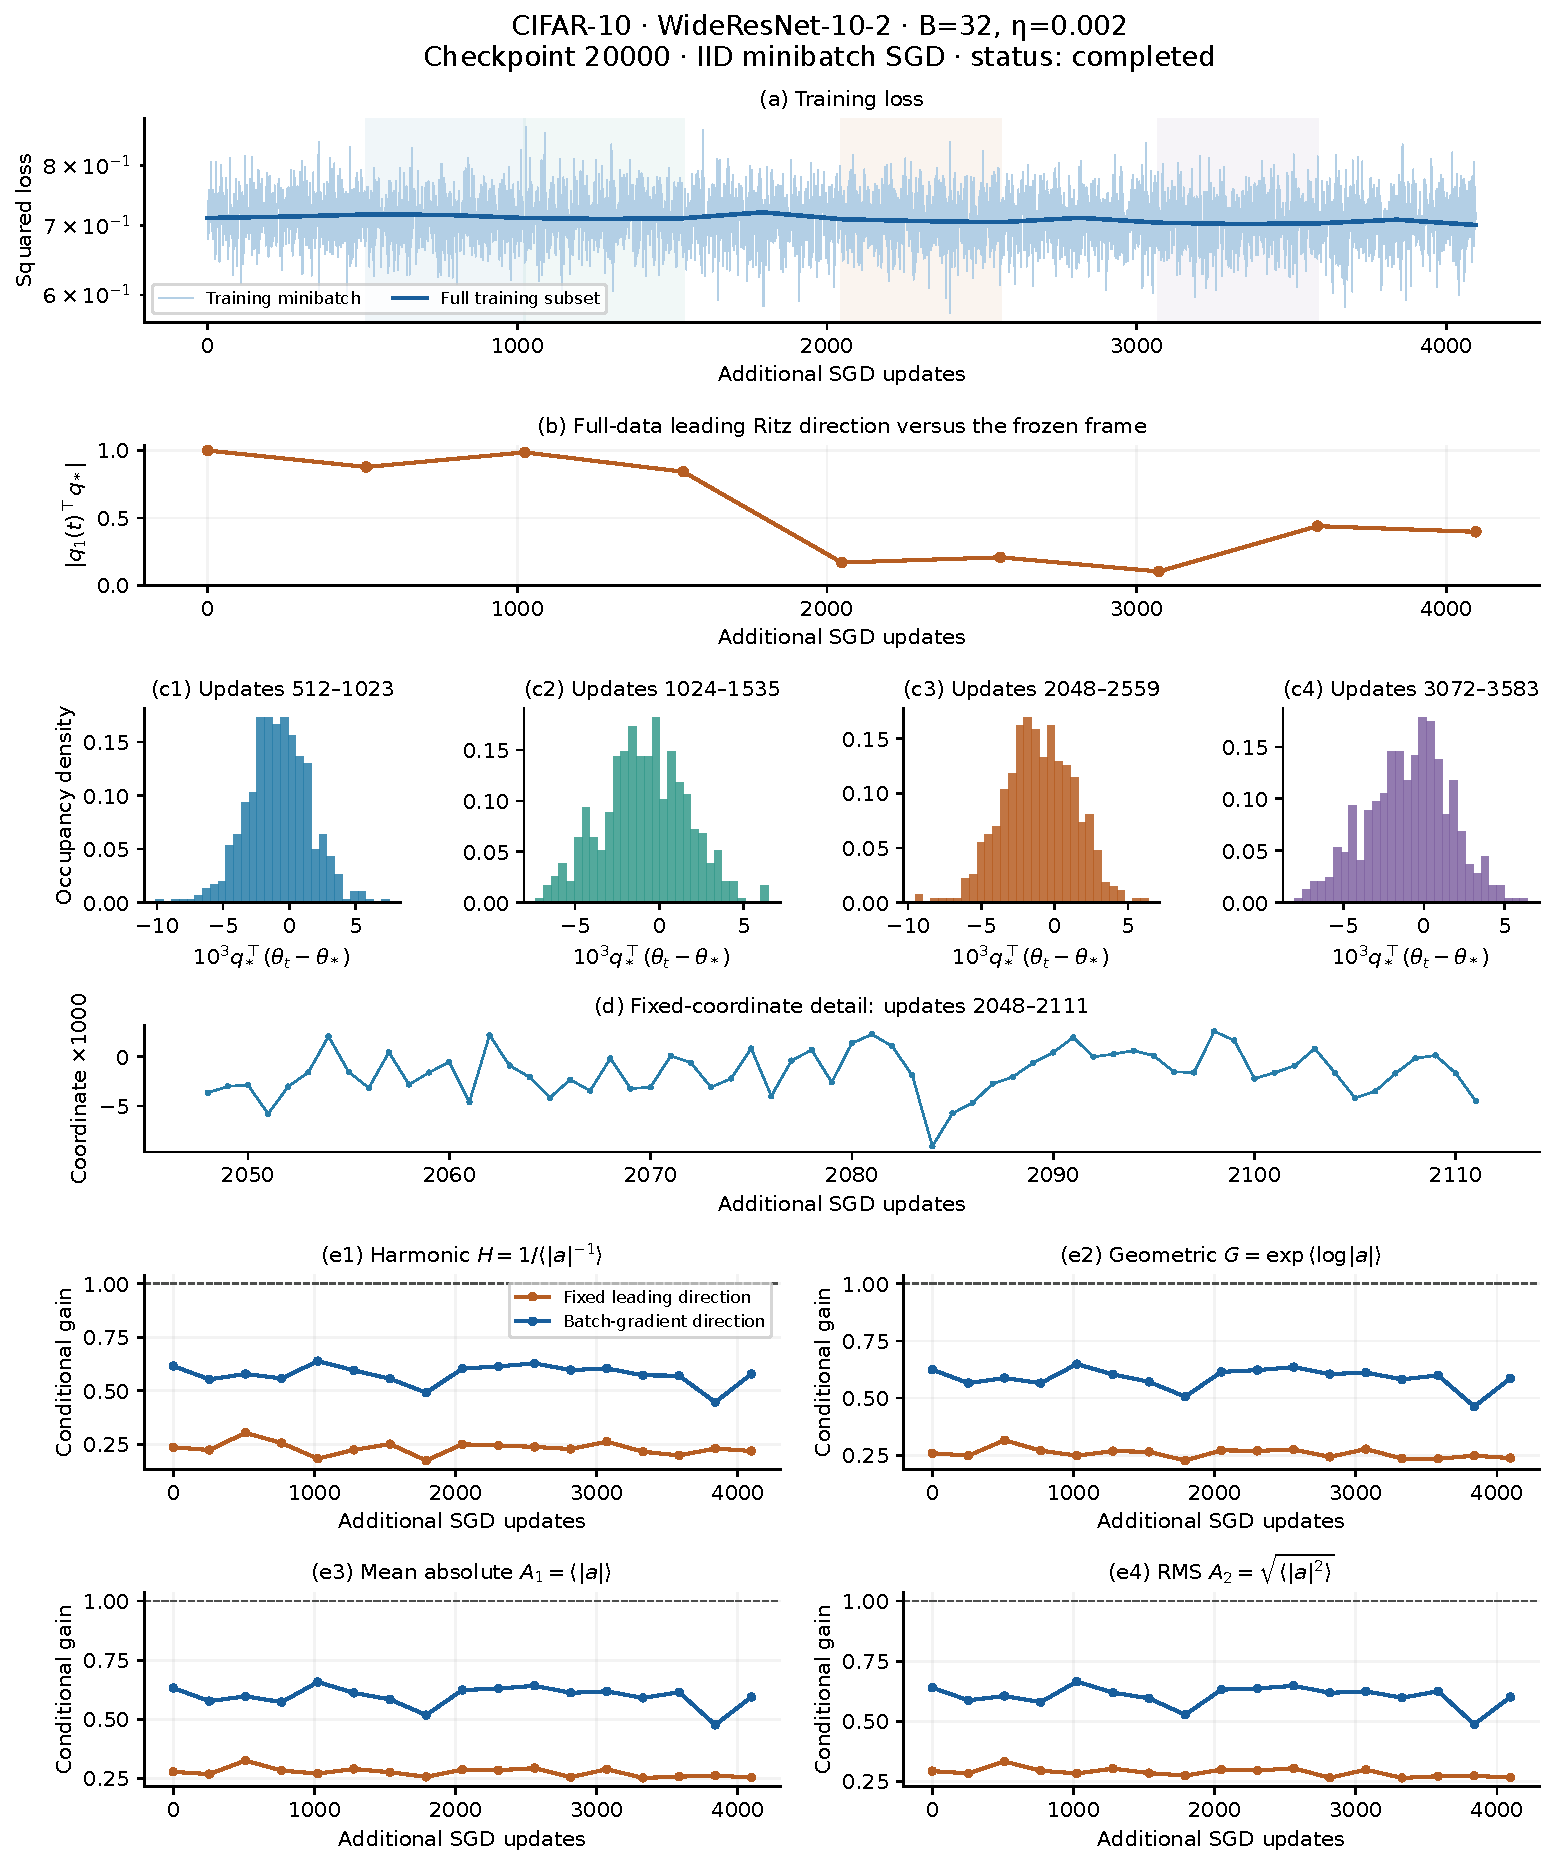
\includegraphics[width=\linewidth,height=0.77\textheight,keepaspectratio]{img/appendix_directional_ladders/wrn_no_bn_B32.pdf}
\caption{\textbf{WideResNet-10-2, batch 32, learning rate 0.002, parent checkpoint 20000.} Loss is shown for both training minibatches and the full 8192-example training subset. The plotting direction $q_*$ and center $\theta_*$ stay fixed at the parent checkpoint; $\theta_*$ is not a verified minimizer. Alignment with separately recomputed leading Hessian Ritz vectors is measured on the full subset, not assumed. Four declared 512-update windows and one 64-update detail are displayed without selection by modality. The lower four panels show fresh conditional scalar gains, comparing $a_{*,B}=1-\eta q_*^\top H_Bq_*$ and $a_{g,B}=1-\eta g_B^\top H_Bg_B/(g_B^\top g_B)$. Their summaries are $H=1/\langle|a|^{-1}\rangle$, $G=\exp\langle\log|a|\rangle$, $A_1=\langle|a|\rangle$, and $A_2=\sqrt{\langle|a|^2\rangle}$, all with reference one. Except for the original anchor, each state has 64 fresh probes every256 updates; the anchor uses 128 probes initially and24 every512 updates. Only even-update states appear here; no phase-averaged or stationary claim follows. No inverse-gain floor is applied.}
\end{figure}\clearpage
\begin{figure}[p]\centering
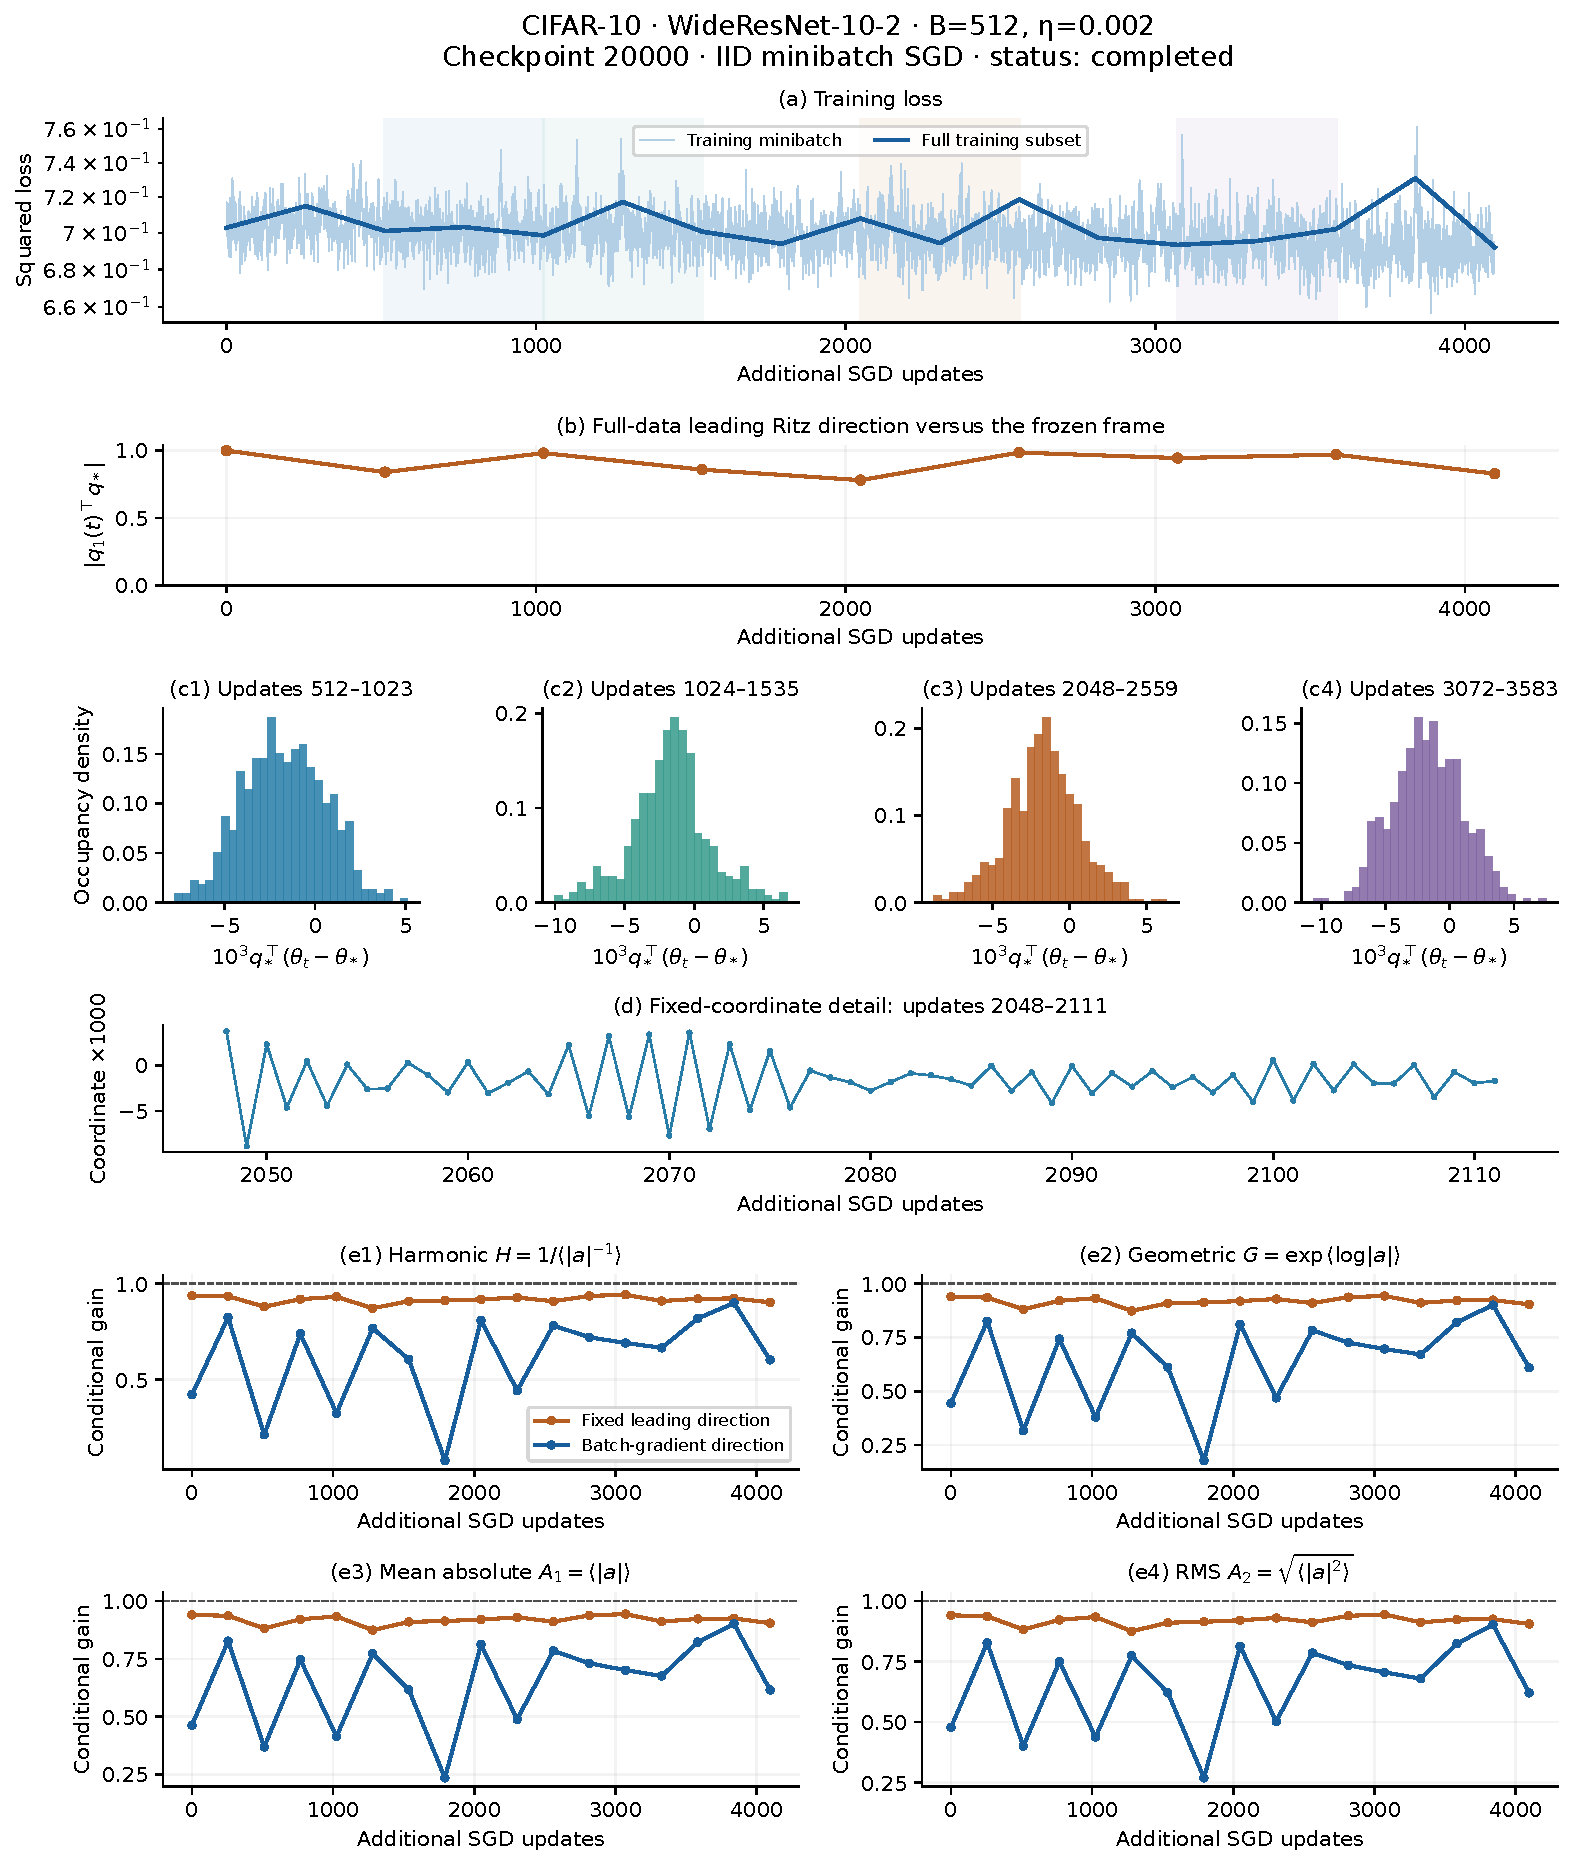
\includegraphics[width=\linewidth,height=0.77\textheight,keepaspectratio]{img/appendix_directional_ladders/wrn_no_bn_B512.pdf}
\caption{\textbf{WideResNet-10-2, batch 512, learning rate 0.002, parent checkpoint 20000.} Loss is shown for both training minibatches and the full 8192-example training subset. The plotting direction $q_*$ and center $\theta_*$ stay fixed at the parent checkpoint; $\theta_*$ is not a verified minimizer. Alignment with separately recomputed leading Hessian Ritz vectors is measured on the full subset, not assumed. Four declared 512-update windows and one 64-update detail are displayed without selection by modality. The lower four panels show fresh conditional scalar gains, comparing $a_{*,B}=1-\eta q_*^\top H_Bq_*$ and $a_{g,B}=1-\eta g_B^\top H_Bg_B/(g_B^\top g_B)$. Their summaries are $H=1/\langle|a|^{-1}\rangle$, $G=\exp\langle\log|a|\rangle$, $A_1=\langle|a|\rangle$, and $A_2=\sqrt{\langle|a|^2\rangle}$, all with reference one. Except for the original anchor, each state has 64 fresh probes every256 updates; the anchor uses 128 probes initially and24 every512 updates. Only even-update states appear here; no phase-averaged or stationary claim follows. No inverse-gain floor is applied.}
\end{figure}\clearpage
